\chapter{Data and Methods}
Much of this thesis relies on the analysis of earthquake catalogs which, along with raw waveforms, are the basic unit of seismology. A number of methods are used in this thesis, both by me and by colleagues and supervisors, in order to derive a catalog of seismicity from raw, unfiltered waveforms recorded at a seismograph stations. This chapter aims to describe the steps taken to create the earthquake catalog analyzed in each of the subsequent chapters. At its most basic, our earthquake catalog for Rotokawa and Ngatamariki contains information about the time of occurrence, location of the event, magnitude of the event and, in some cases, information about how the fault or fracture slipped (focal mechanisms). What follows is a description of the methods of detection, location, magnitude estimation and focal mechanism determination starting from raw waveforms.

Apart from seismic data, a number of other data streams are used in this thesis for the purpose of assessing the relationship between seismicity and geothermal field operations. These data are touched upon in Chapter 1, but those with the greatest significance to this work will be detailed here. Specifically, well pressure, temperature and flow rate measurements are used extensively both for direct comparison to rates of seismicity and also to make inferences about the reservoir. 

\section{Data}
\subsection{Seismic network}
The seismic data presented in this thesis were recorded on a network of between 15 and 29 seismometers, most of which are concentrated in an area 15 km N-S by 7 km E-W centered around the Rotokawa and Ngatamariki geothermal fields (Figure \ref{322599}). The vast majority of the stations are owned and operated by Mercury NZ Ltd., for the purpose of monitoring the geothermal fields. However, six stations from either Contact Energy (ARAZ, THQ2) or GeoNet, the national seismic network (HRRZ, PRRZ, ALRZ, WPRZ), have been incorporated into this network to improve station coverage.

GNS Science in Waikarei has been contracted to maintain the seismic network at the geothermal fields, a task which includes quarterly retrieval of data, which is stored locally at each station between servicing trips. As detailed in Table \ref{station_table}, the Mercury-operated stations are 4.5 Hz geophones and the data are sampled at 200 Hz. Three of these stations are borehole instruments (NS12, NS13, NS14), deployed in the center of the Ngatamariki field at depths of between 202 and 514 m. The GeoNet data are sampled at 100 Hz and were downloaded and archived locally at the outset of this project in order to speed up analysis.

As the Rotokawa reservoir has been developed for considerably longer than Ngatamariki, its seismic network (stations named RT) has been in operation for over a decade. Ngatamariki stations began to be installed prior to drilling operations in mid-2012. Network coverage varied with time as certain stations were moved to improve performance or replaced after damage due to livestock or vandalism. Therefore, the network presented in Figure \ref{322599} does not represent the exact geometry for any specific point in time, instead reflecting the locations of instruments that were operational at any point between 2012 and 2015.\selectlanguage{english}
\begin{figure}[h!]
\begin{center}
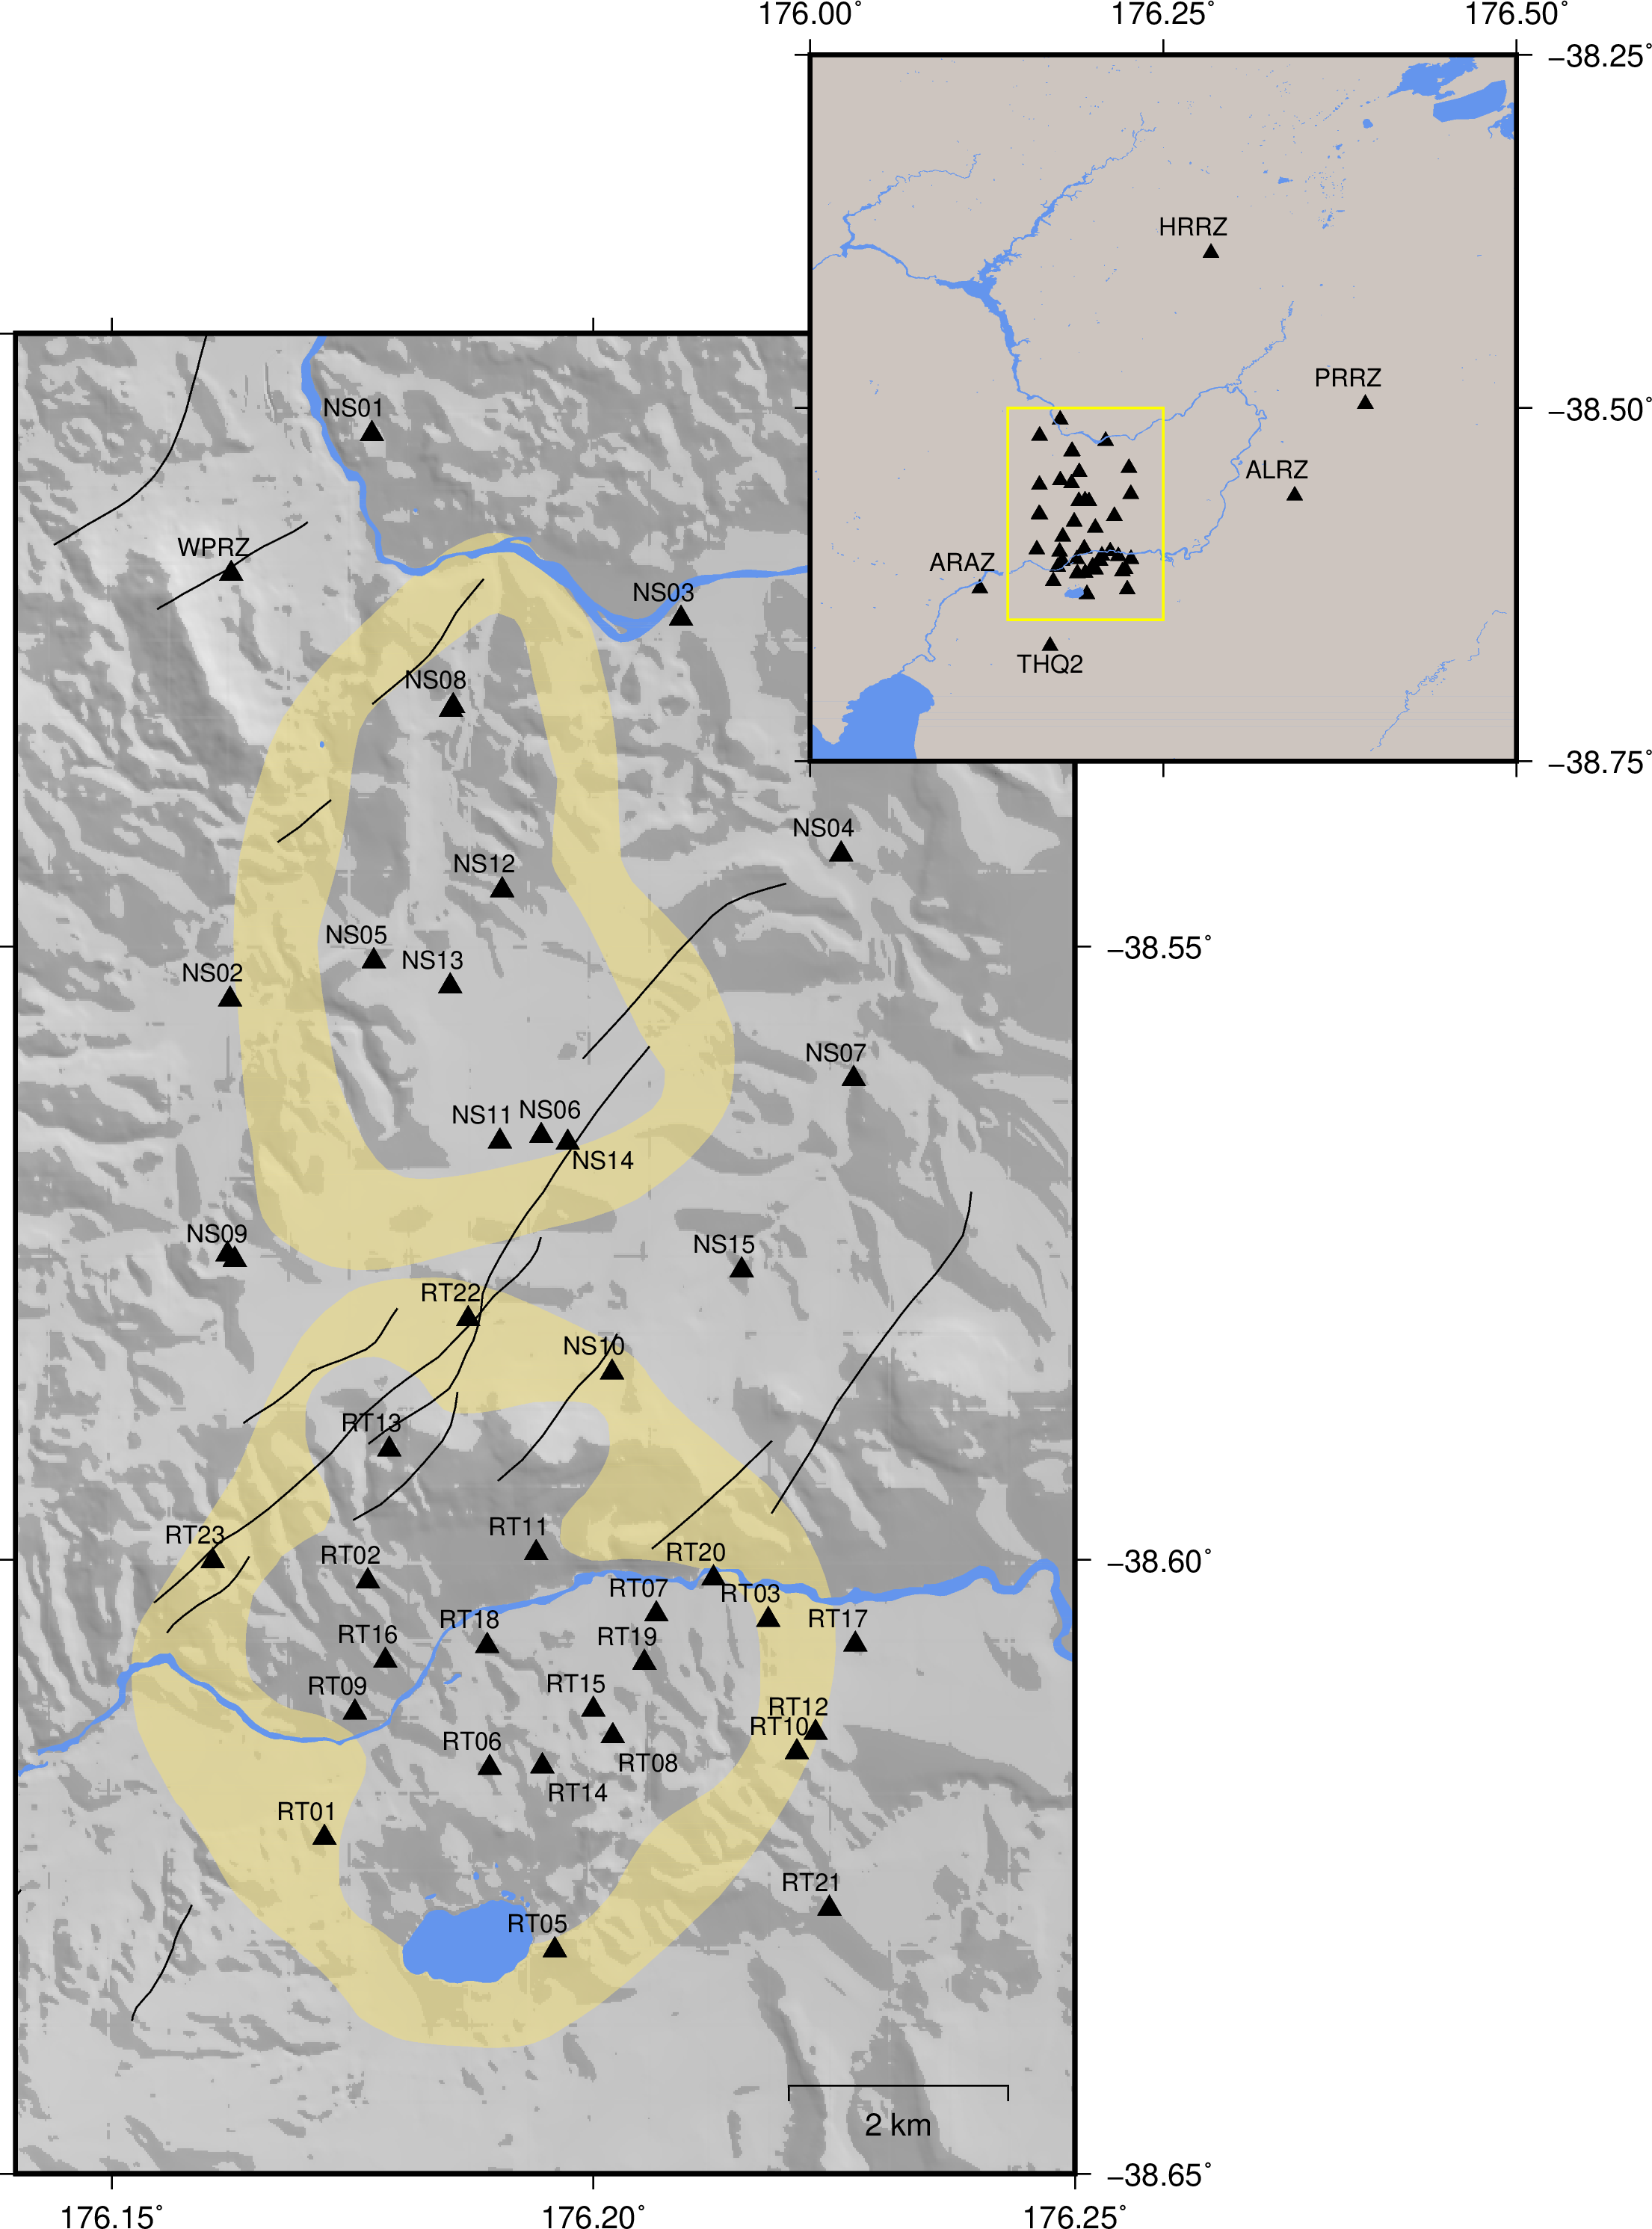
\includegraphics[width=0.70\columnwidth]{Chapter_2_Data/figures/RotNga_stations_overview/RotNga_stations_overview_original}
\caption{{All stations that were active at any time between 2012 and 2015.
Goldenrod shapes indicate the most likely resistivity boundaries for the
Ngatamariki and Rotokawa geothermal fields, triangles show the locations
of seismic stations, each of which is labeled with the station name
appearing in Table 1, below.
{\label{322599}}%
}}
\end{center}
\end{figure}\selectlanguage{english}
\begin{table}
\centering
\resizebox{\textwidth}{!}{%
\begin{tabular}{cccccc}
    {Station name} & {Longitude} & {Latitude} & {Elevation (m)} & {Depth (m)} & {Sensor} \\ \midrule
    ALRZ & 176.343014 & -38.562043 & 405.0 & 0.0 & L4C-3D \\
    ARAZ & 176.12006 & -38.62769 & 420.0 & 0.0 & L4C-3D \\
    HRRZ & 176.283754 & -38.39013 & 590.0 & 0.0 & L4C-3D \\
    NS01 & 176.177 & -38.5082 & 349.0 & 0.0 & Geospace GS-11D \\
    NS02 & 176.162275 & -38.554318 & 375.0 & 0.0 & Geospace GS-11D \\
    NS03 & 176.209102 & -38.523259 & 327.0 & 0.0 & Geospace GS-11D \\
    NS04 & 176.225718 & -38.542487 & 345.0 & 0.0 & Geospace GS-11D \\
    NS05 & 176.1772 & -38.5512 & 386.0 & 0.0 & Geospace GS-11D \\
    NS06 & 176.194571 & -38.565449 & 407.0 & 0.0 & Geospace GS-11D \\
    NS07 & 176.227019 & -38.560793 & 345.0 & 0.0 & Geospace GS-11D \\
    NS08 & 176.185438 & -38.530393 & 345.0 & 0.0 & Geospace GS-11D \\
    NS09 & 176.162759 & -38.575539 & 451.0 & 0.0 & Geospace GS-11D \\
    NS10 & 176.201928 & -38.584723 & 400.0 & 0.0 & Geospace GS-11D \\
    NS11 & 176.1903 & -38.5659 & 409.0 & 0.0 & Geospace GS-11D \\
    NS12 & 176.190524 & -38.545408 & 350.0 & 514.0 & IESE Borehole: Duke 4.5 \\
    NS13 & 176.185137 & -38.553235 & 380.0 & 250.0 & IESE Borehole: Duke 4.5 \\
    NS14 & 176.197332 & -38.565986 & 365.0 & 202.0 & IESE Borehole: Duke 4.5 \\
    NS15 & 176.2154 & -38.5764 & 382.0 & 0.0 & Geospace GS-11D \\
    NS16 & 176.162 & -38.5751 & 450.0 & 0.0 & Geospace GS-11D \\
    NS18 & 176.1852 & -38.5307 & 348.0 & 0.0 & Geospace GS-11D \\
    PRRZ & 176.393 & -38.4971 & 392.0 & 0.0 & L4C-3D \\
    RT01 & 176.17208 & -38.62264 & 371.0 & 0.0 & LE-3Dlite \\
    RT02 & 176.17658 & -38.60173 & 346.0 & 0.0 & LE-3Dlite \\
    RT03 & 176.21815 & -38.60488 & 337.0 & 0.0 & LE-3Dlite \\
    RT05 & 176.19599 & -38.63178 & 369.0 & 0.0 & LE-3Dlite \\
    RT06 & 176.18922 & -38.61694 & 366.0 & 0.0 & LE-3Dlite \\
    RT07 & 176.20653 & -38.60443 & 320.0 & 0.0 & LE-3Dlite \\
    RT08 & 176.20201 & -38.61436 & 341.0 & 0.0 & LE-3Dlite \\
    RT09 & 176.17524 & -38.61243 & 339.0 & 0.0 & Geospace GS-11D \\
    RT10 & 176.22112 & -38.61567 & 408.0 & 0.0 & Geospace GS-11D \\
    RT11 & 176.194057 & -38.599442 & 330.0 & 0.0 & Geospace GS-11D \\
    RT12 & 176.223066 & -38.614089 & 400.0 & 0.0 & Geospace GS-11D \\
    RT13 & 176.1788 & -38.591 & 428.0 & 0.0 & Geospace GS-11D \\
    RT14 & 176.1947 & -38.6168 & 380.0 & 0.0 & Geospace GS-11D \\
    RT15 & 176.2 & -38.6122 & 352.0 & 0.0 & Geospace GS-11D \\
    RT16 & 176.1784 & -38.6082 & 336.0 & 0.0 & Geospace GS-11D \\
    RT17 & 176.2272 & -38.6069 & 342.0 & 0.0 & Geospace GS-11D \\
    RT18 & 176.188968 & -38.606998 & 308.0 & 0.0 & Geospace GS-11D \\
    RT19 & 176.205294 & -38.608375 & 312.0 & 0.0 & Geospace GS-11D \\
    RT20 & 176.212467 & -38.601494 & 300.0 & 0.0 & Geospace GS-11D \\
    RT21 & 176.2245 & -38.6284 & 250.0 & 0.0 & Geospace GS-11D \\
    RT22 & 176.186985 & -38.580367 & 423.0 & 0.0 & Geospace GS-11D \\
    RT23 & 176.160466 & -38.600085 & 447.0 & 0.0 & Geospace GS-11D \\
    THQ2 & 176.1698 & -38.6684 & 450.0 & 80.0 & IESE Borehole: Duke 4.5 \\
    WPRZ & 176.1624 & -38.5196 & 519.0 & 0.0 & LE-3DliteMkII \\
\end{tabular}}
\caption{{Summary of each station active at any time between 2012 and 2015 at Rotokawa and Ngatamariki. Most stations are owned and operated by Mercury NZ Ltd. However, stations ARAZ and THQ2 are owned and operated by Contact Energy and stations ALRZ, HRRZ, PRRZ and WPRZ are operated by the national seismic network, GeoNet.}}
\label{station_table}
\end{table}

\subsection{Preliminary earthquake catalog}\label{GNS_cat}
As stated above, the initial earthquake catalog was constructed by GNS Science using the software package SeisComP3 \citep{Weber2007}. Event detection was done using a short-term average\slash{long-term average} technique, which records a detection when the ratio of the average amplitude in a user-defined, short-term window to that in a long-term window exceeds a threshold value. Each of these detections was then automatically located using the linearized location algorithm Hypo71 \citep{Lee_1972}. See Sections \ref{STA/LTA} and \ref{linloc} for a detailed description of these techniques.

Local magnitudes were also calculated using the SeisComP3 module \textit{scmag}, which uses the ubiquitous equation from Richter \citep{richter1935instrumental} for magnitude at an individual station:

\begin{equation}
M_L = \log_{10}{A} - \log_{10}A0
\end{equation}

where $A$ is the amplitude of the seismic trace in mm and $A0$ is a calibration term that is used to adjust the scale to different localities. In this case, the SeisComP3 \textit{logA0} module was used with distance calibration values of $A0$ summarized in Table \ref{table_A0}. The magnitudes at each station were averaged to return the final event magnitude.\selectlanguage{english}
\begin{table}
\centering
\begin{tabular}{cc}
    {Event-station dist (km)} & {Calibration (mag. units)} \\ \midrule
    0  & 0.0431 \\
    10  & -1.1563  \\
    50  & -1.5755  \\
    100  & -1.7560  \\
    1000  & -2.3545   \\
\end{tabular}
\caption{{Table summarizing the distance correction factors used by GNS Science in calculating the magnitudes of the preliminary earthquake catalog.}}
\label{table_A0}
\end{table}

The national seismic network, GeoNet, reports location and magnitude information for most earthquakes above magnitude 2.1 in the area of Rotokawa and Ngatamariki \citep{Sherburn_2015}. The GeoNet-calculated magnitudes of such events at the geothermal fields were compared with the independently-calculated magnitudes from the stations in the Mercury network used in this study (note that three stations from the GeoNet network were included in the Mercury seismic network). There was found to be a disagreement between GeoNet- and Mercury-calculated magnitudes of -0.32 magnitude units, which was addressed by applying a static correction of +0.32 to all Mercury-network magnitudes in the preliminary catalog used in this thesis. The corrected magnitudes are compared to the GeoNet magnitudes in Figure \ref{910533}, showing that the relationship between the two sets of magnitudes is approximately 1:1.\selectlanguage{english}

\begin{figure}[h!]
\begin{center}
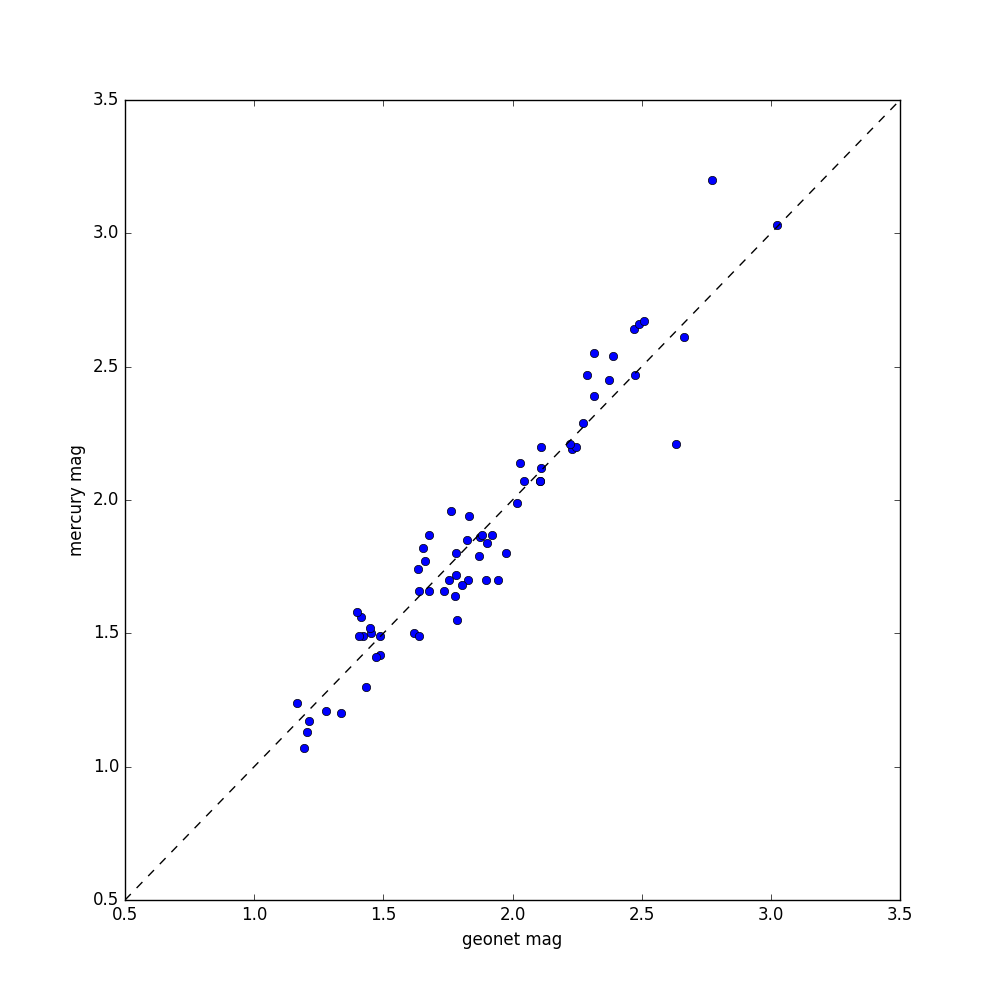
\includegraphics[width=0.70\columnwidth]{Chapter_2_Data/figures/geonet-merc_mag_comp/geonet-merc_mag_comp_original}
\caption{{Mercury-calculated vs GeoNet calculated magnitudes after applying a
static correction of +0.32 magnitude units to the Mercury events.
{\label{910533}}%
}}
\end{center}
\end{figure}

Following the steps outlined above, GNS Science provided us the Rotokawa\slash{Ngatamariki} earthquake catalog in the form of SeisComP3 native \textit{sc3ml} xml files. This catalog contained 8226 earthquakes that occurred between 15 May 2012 and 18 November 2015 (black events, Figure \ref{955268}). These two dates correspond to the date of the start of the first Ngatamariki seismographs, at which time the Rotokawa and Ngatamariki seismic networks were combined, and the final data-collection date of 2015, respectively. Many of these events occurred outside of the boundaries of the geothermal fields and were therefore marginally applicable to the aims of this thesis. For this reason, we filtered the catalog to include only events that occurred within or adjacent the field boundaries of Rotokawa and Ngatamariki, and also to include events with average pick residuals within one standard deviation of the mean, leaving a total of 4405 events (Figure \ref{955268}). These earthquakes were used as 'template' events in detecting additional events as detailed in Section \ref{MF} below.\selectlanguage{english}

\begin{figure}[h!]
\begin{center}
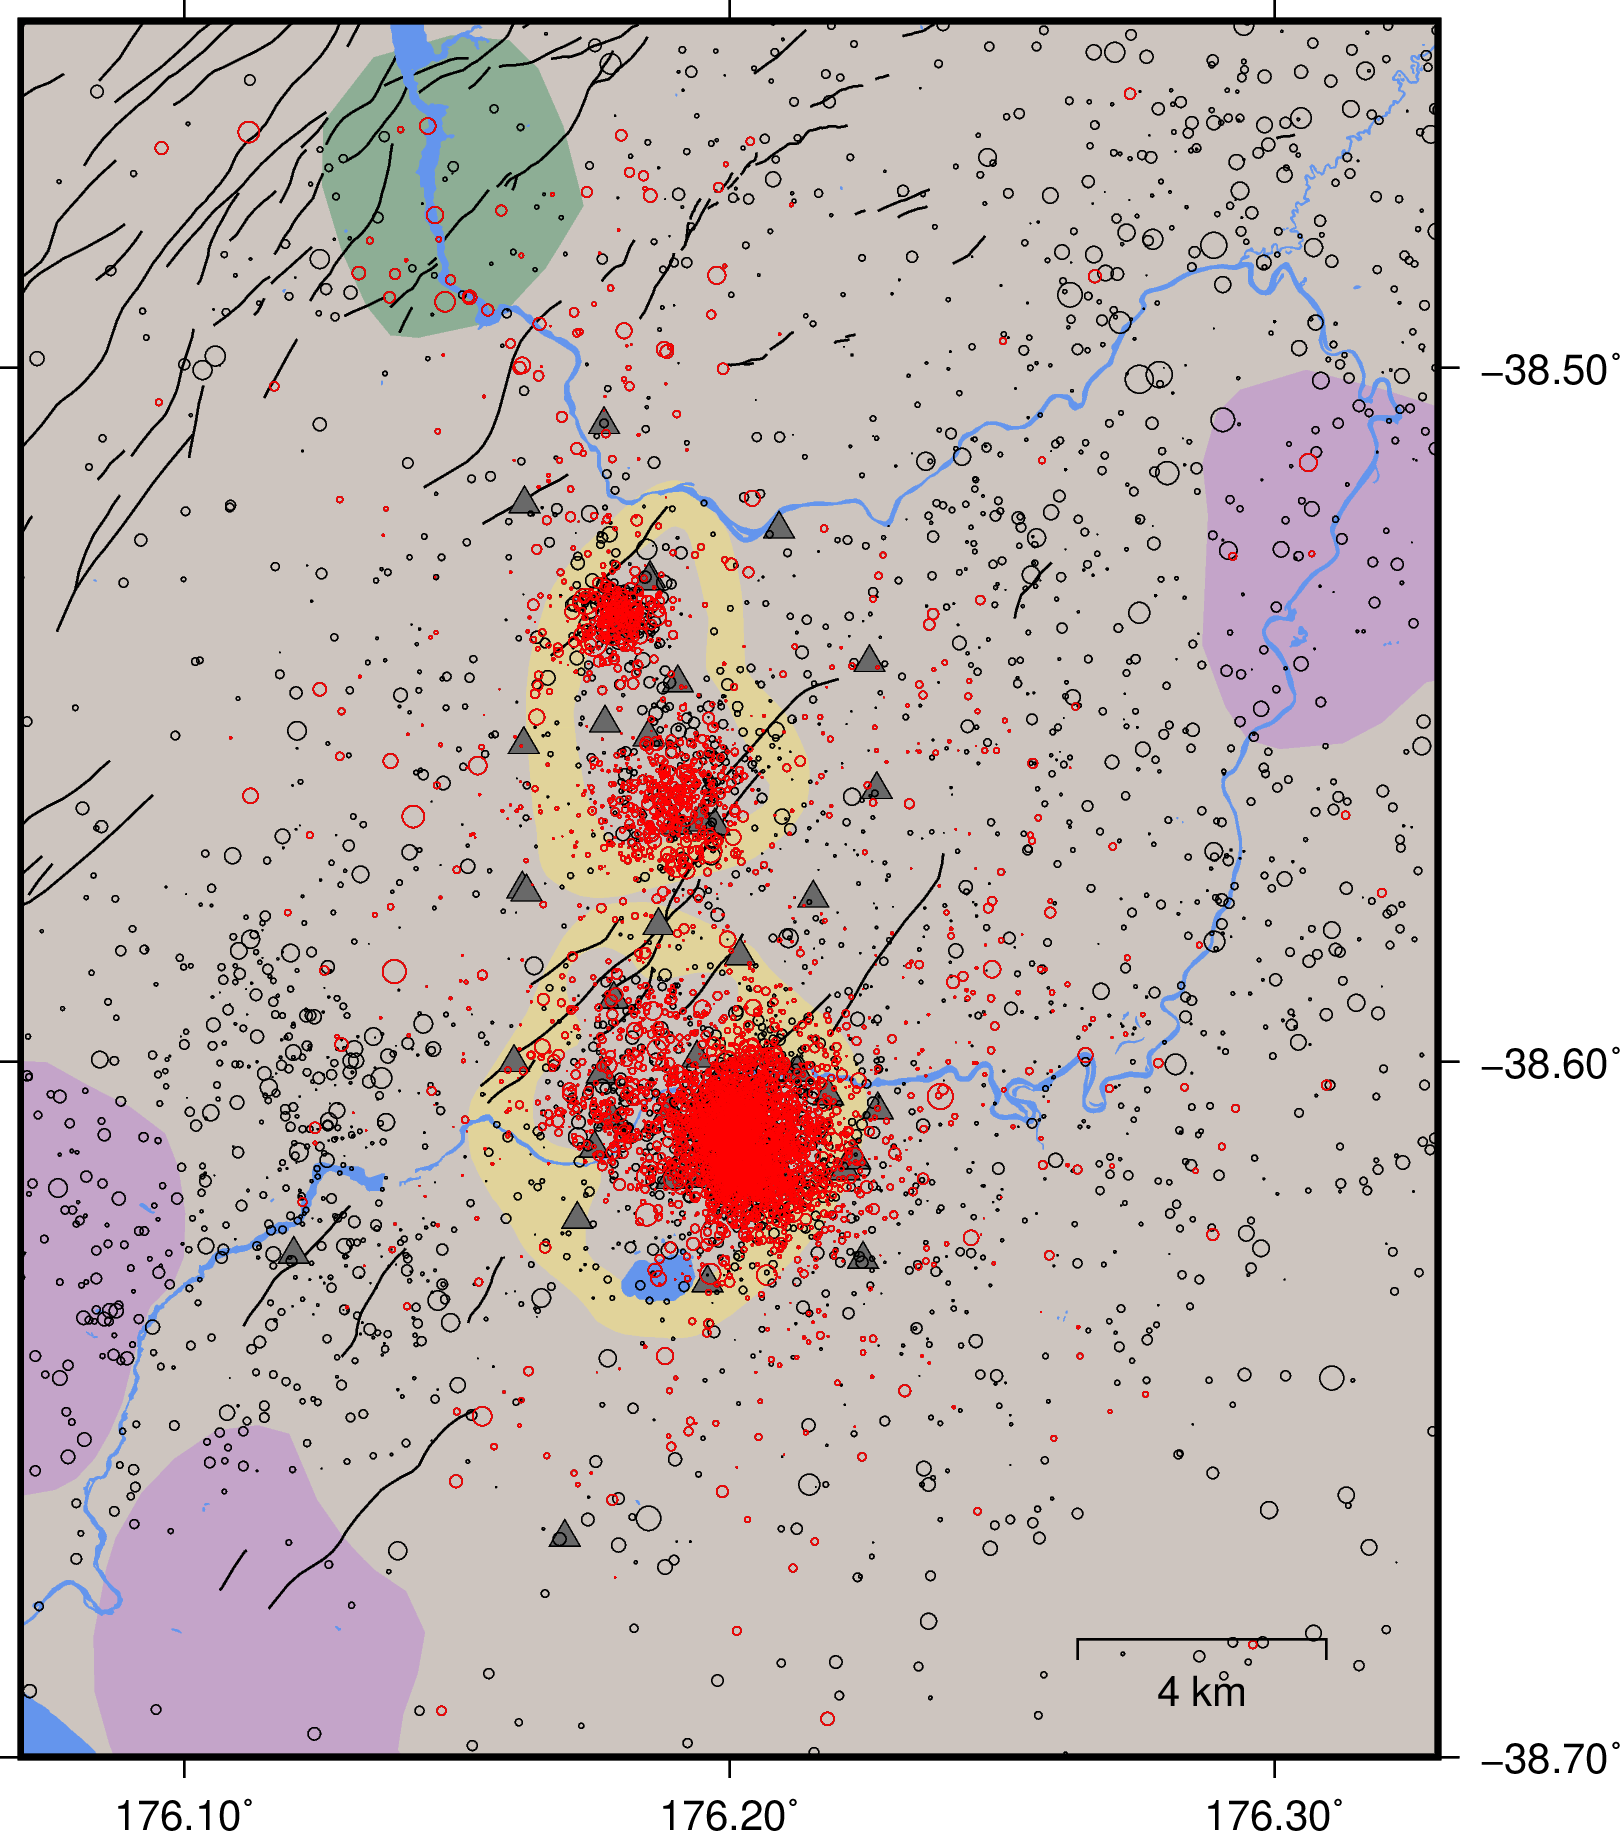
\includegraphics[width=0.70\columnwidth]{Chapter_2_Data/figures/RotNga_catalog_overview/RotNga_catalog_overview_original}
\caption{{Overview of earthquakes in the preliminary GNS Science catalog. Red
events are those which were selected for use in the analyses detailed in
the following sections. Gray triangles represent seismograph stations.
Yellow indicates the boundaries of the Ngatamariki and Rotokawa
geothermal fields, purple nearby Contact Energy-operated fields, and
green the protected Orakei-Korako geothermal field. Black lines show
active faults. Event symbols are scaled by magnitude where the largest
is magnitude 4.2.
{\label{955268}}%
}}
\end{center}
\end{figure}

\subsection{Mercury datasets}
In this thesis, we make use of a number of additional datasets that have been provided by Mercury. These data record the industrial processes taking place at the fields (such as injection and extraction of fluids) as well as properties of the deep reservoir that can be directly measured or inferred from the limited number of wells. They also provide important constraints for the interpretation of the earthquake catalog throughout this work.

\subsubsection{Injection and production rates}
The most important supporting datasets are pressure and flow rate time series for all injection and production wells. Specifically, they provide constraint on the reservoir pressures and injected volumes required to trigger or halt nearby seismicity. Flow and pressure time series are sampled daily during normal plant operations at both fields and more frequently during completion\slash{stimulation} tests at Ngatamariki (usually every five minutes). Pressure measurements can be taken either at the wellhead, in which case is they are referred to as wellhead pressure (WHP) or at depth from within the wellbore, which is referred to as downhole pressure (DHP). Example flow rate and pressure data are shown in the introductory chapter.

\subsubsection{Pressure-temperature spinner data}
In practice, fluid does not exit (injection) or enter (production) a well uniformly across its entire length. Differences in permeability, controlled by rock type and fractures\slash{faults} intersecting the well, mean that a well is hydraulically connected to the reservoir only at specific zones. These intervals are referred to as feedzones or permeable zones. In certain cases, operators will install a slotted or perforated liner in the well to dictate specifically where fluid will be able to move into or out of the well, however it is often common in geothermal reservoirs to leave the hole `open' below the casing shoe. Even in the case of a perforated liner, the locations of the principle feedzones are unknown a priori. In order to infer feedzone location, a tool called a pressure-temperature spinner (PTS) is used, which measures flow, pressure and temperature within a well during production or injection. PTS tests are often run as a part of the completion testing of a well (Figure \ref{748181}).\selectlanguage{english}

\begin{sidewaysfigure}[p]
\begin{center}
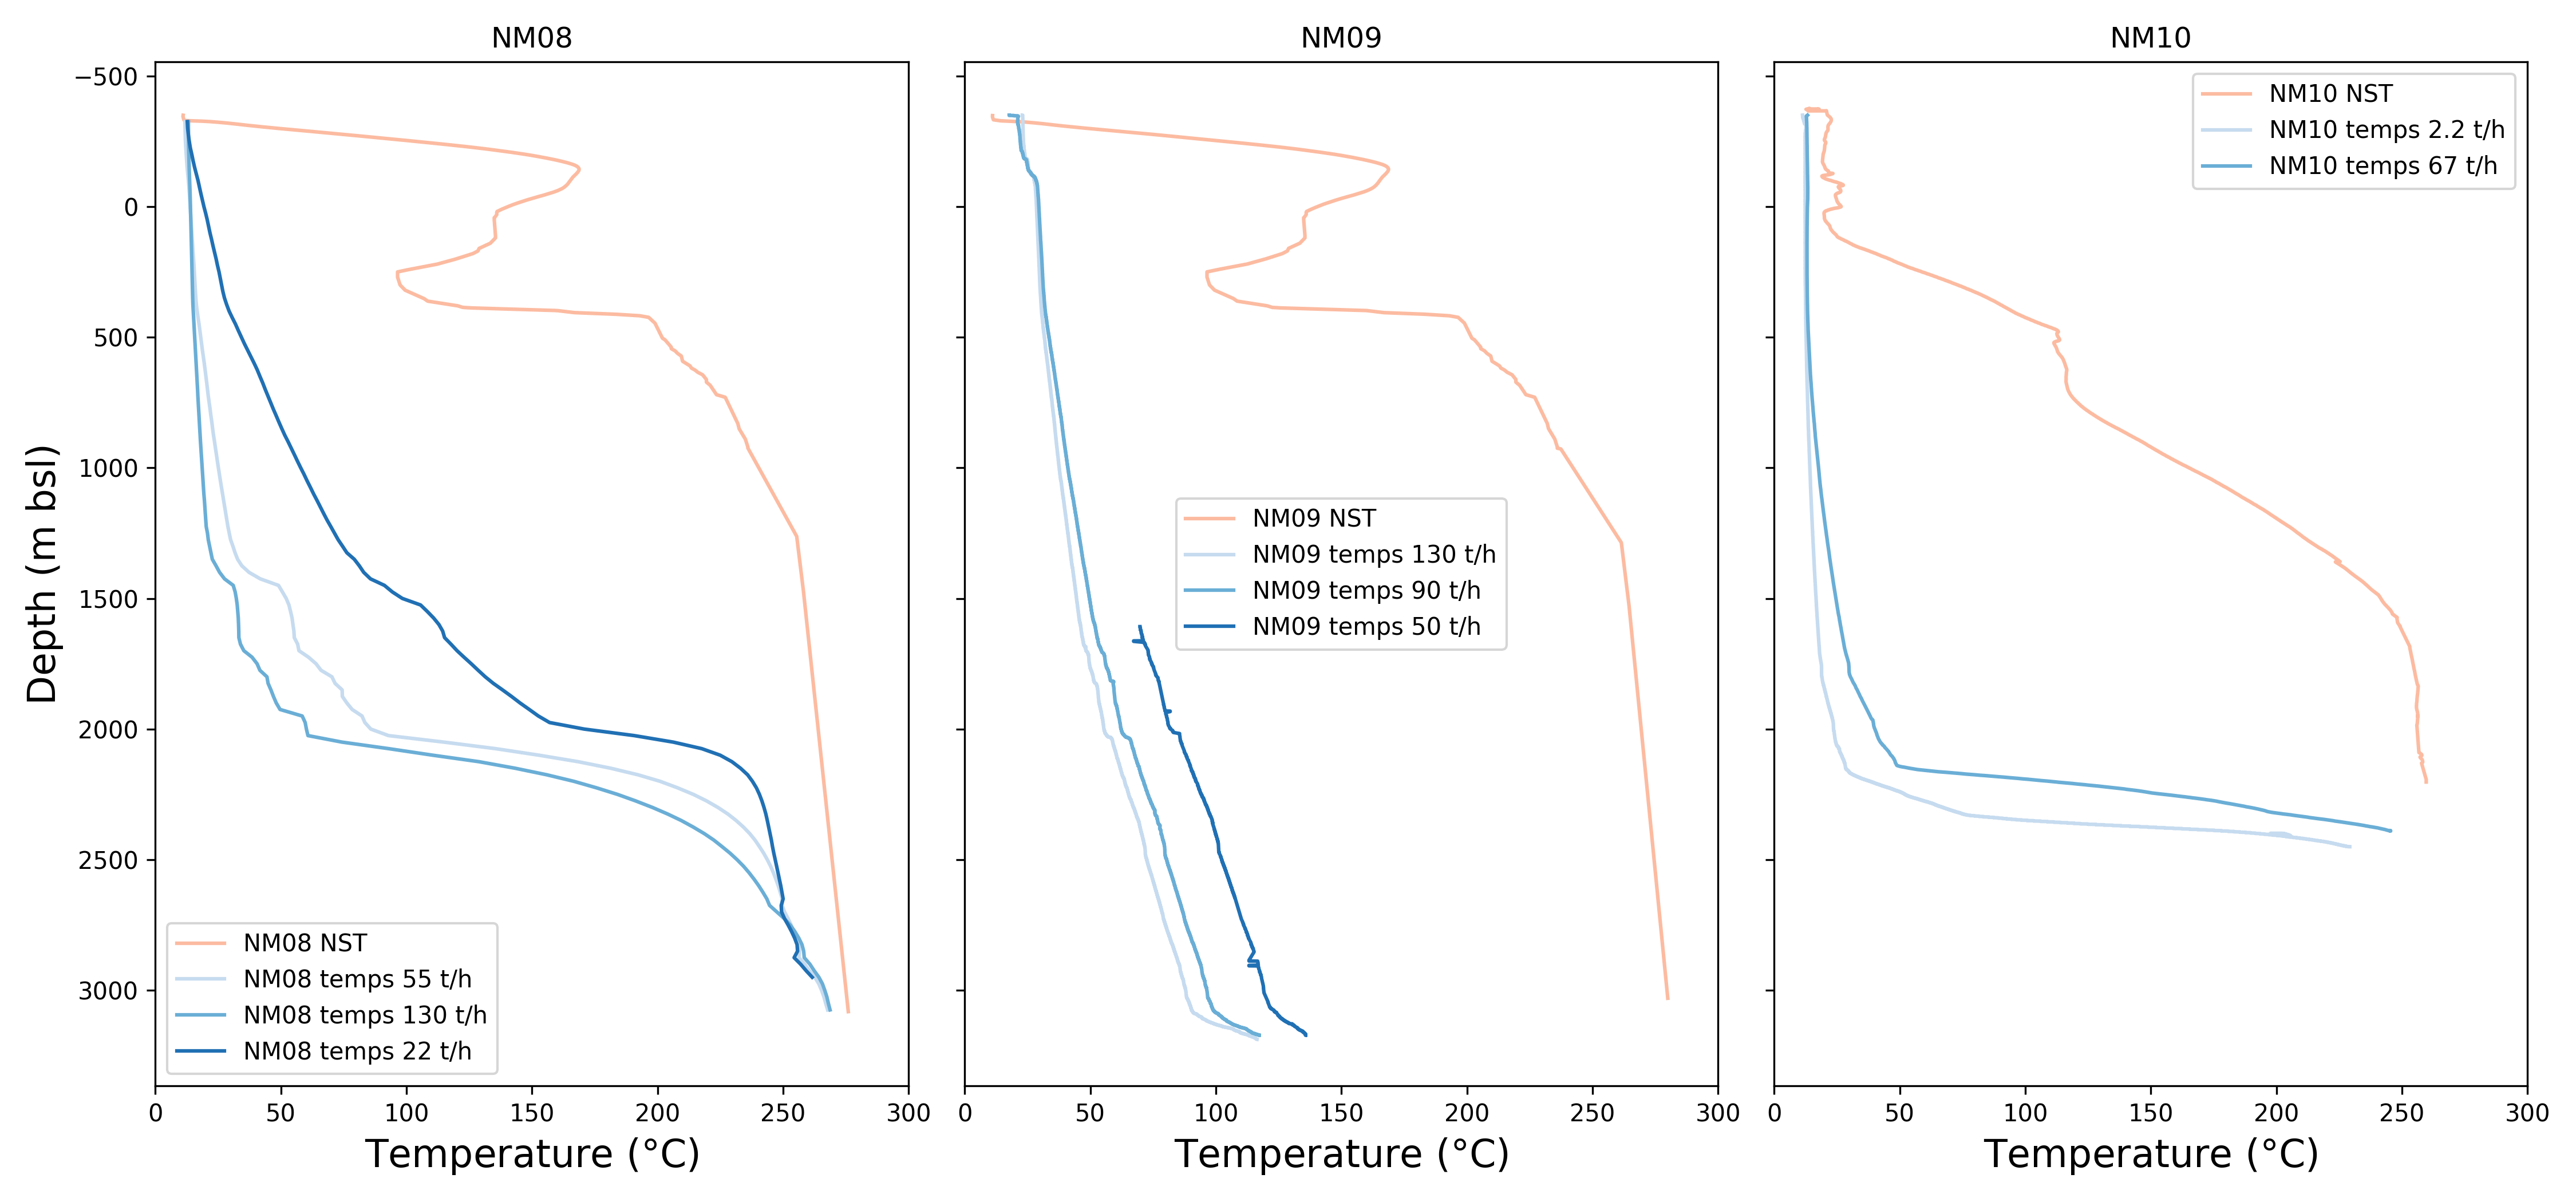
\includegraphics[width=\textwidth,height=\textheight,keepaspectratio]{Chapter_2_Data/figures/all_wells_Nga/all_wells_Nga_original}
\caption{{Pressure-temperature spinner data recorded during completion tests at
each of the three wells drilled at Ngatamariki in 2012. The blue lines
indicate temperatures for fluid injected at various static flow rates
and the orange lines represent combinations of measured and interpreted
natural state temperatures in the reservoir.
{\label{748181}}%
}}
\end{center}
\end{sidewaysfigure}

For a given flow rate, a strong variation in temperature over some depth interval typically implies that fluid is entering or leaving the well and that the corresponding depth may be a feedzone. In the case of the injection tests shown in Figure \ref{748181}, strong `heating' signals with depth signify that a relatively large volume of cold injectate is moving from the well into the reservoir, leaving hotter, conductively-heated fluid in the wellbore at greater depths. This information constrains the points from which fluid flows, and therefore helps us to interpret where pressure signals originate and how they relate to the characteristics of seismicity.

\subsubsection{Image logs}
In the case of many geothermal reservoirs, including Ngatamariki and Rotokawa, permeability is controlled by the reservoir fracture network. This is because the matrix rock is far less permeable than the typically extensive open fractures \citep{Grant_2011,Cant_2018}. A final important constraint on the locations of well feedzones, as well at the distribution and orientation of fractures over the entire reservoir, are resistivity- and sonic-based image logs. These logs are capable of showing detailed structures that intersect the wellbore including open (permeable) and sealed (impermeable) fractures and help corroborate data obtained from PTS measurements as to the location of feedzones (Figure \ref{746257}). These measurements of reservoir fracture orientations are also useful contraints on the structures available to slip, and therefore help to constrain fault plane ambiguity in focal mechanism results.\selectlanguage{english}

\begin{figure}[h!]
\begin{center}
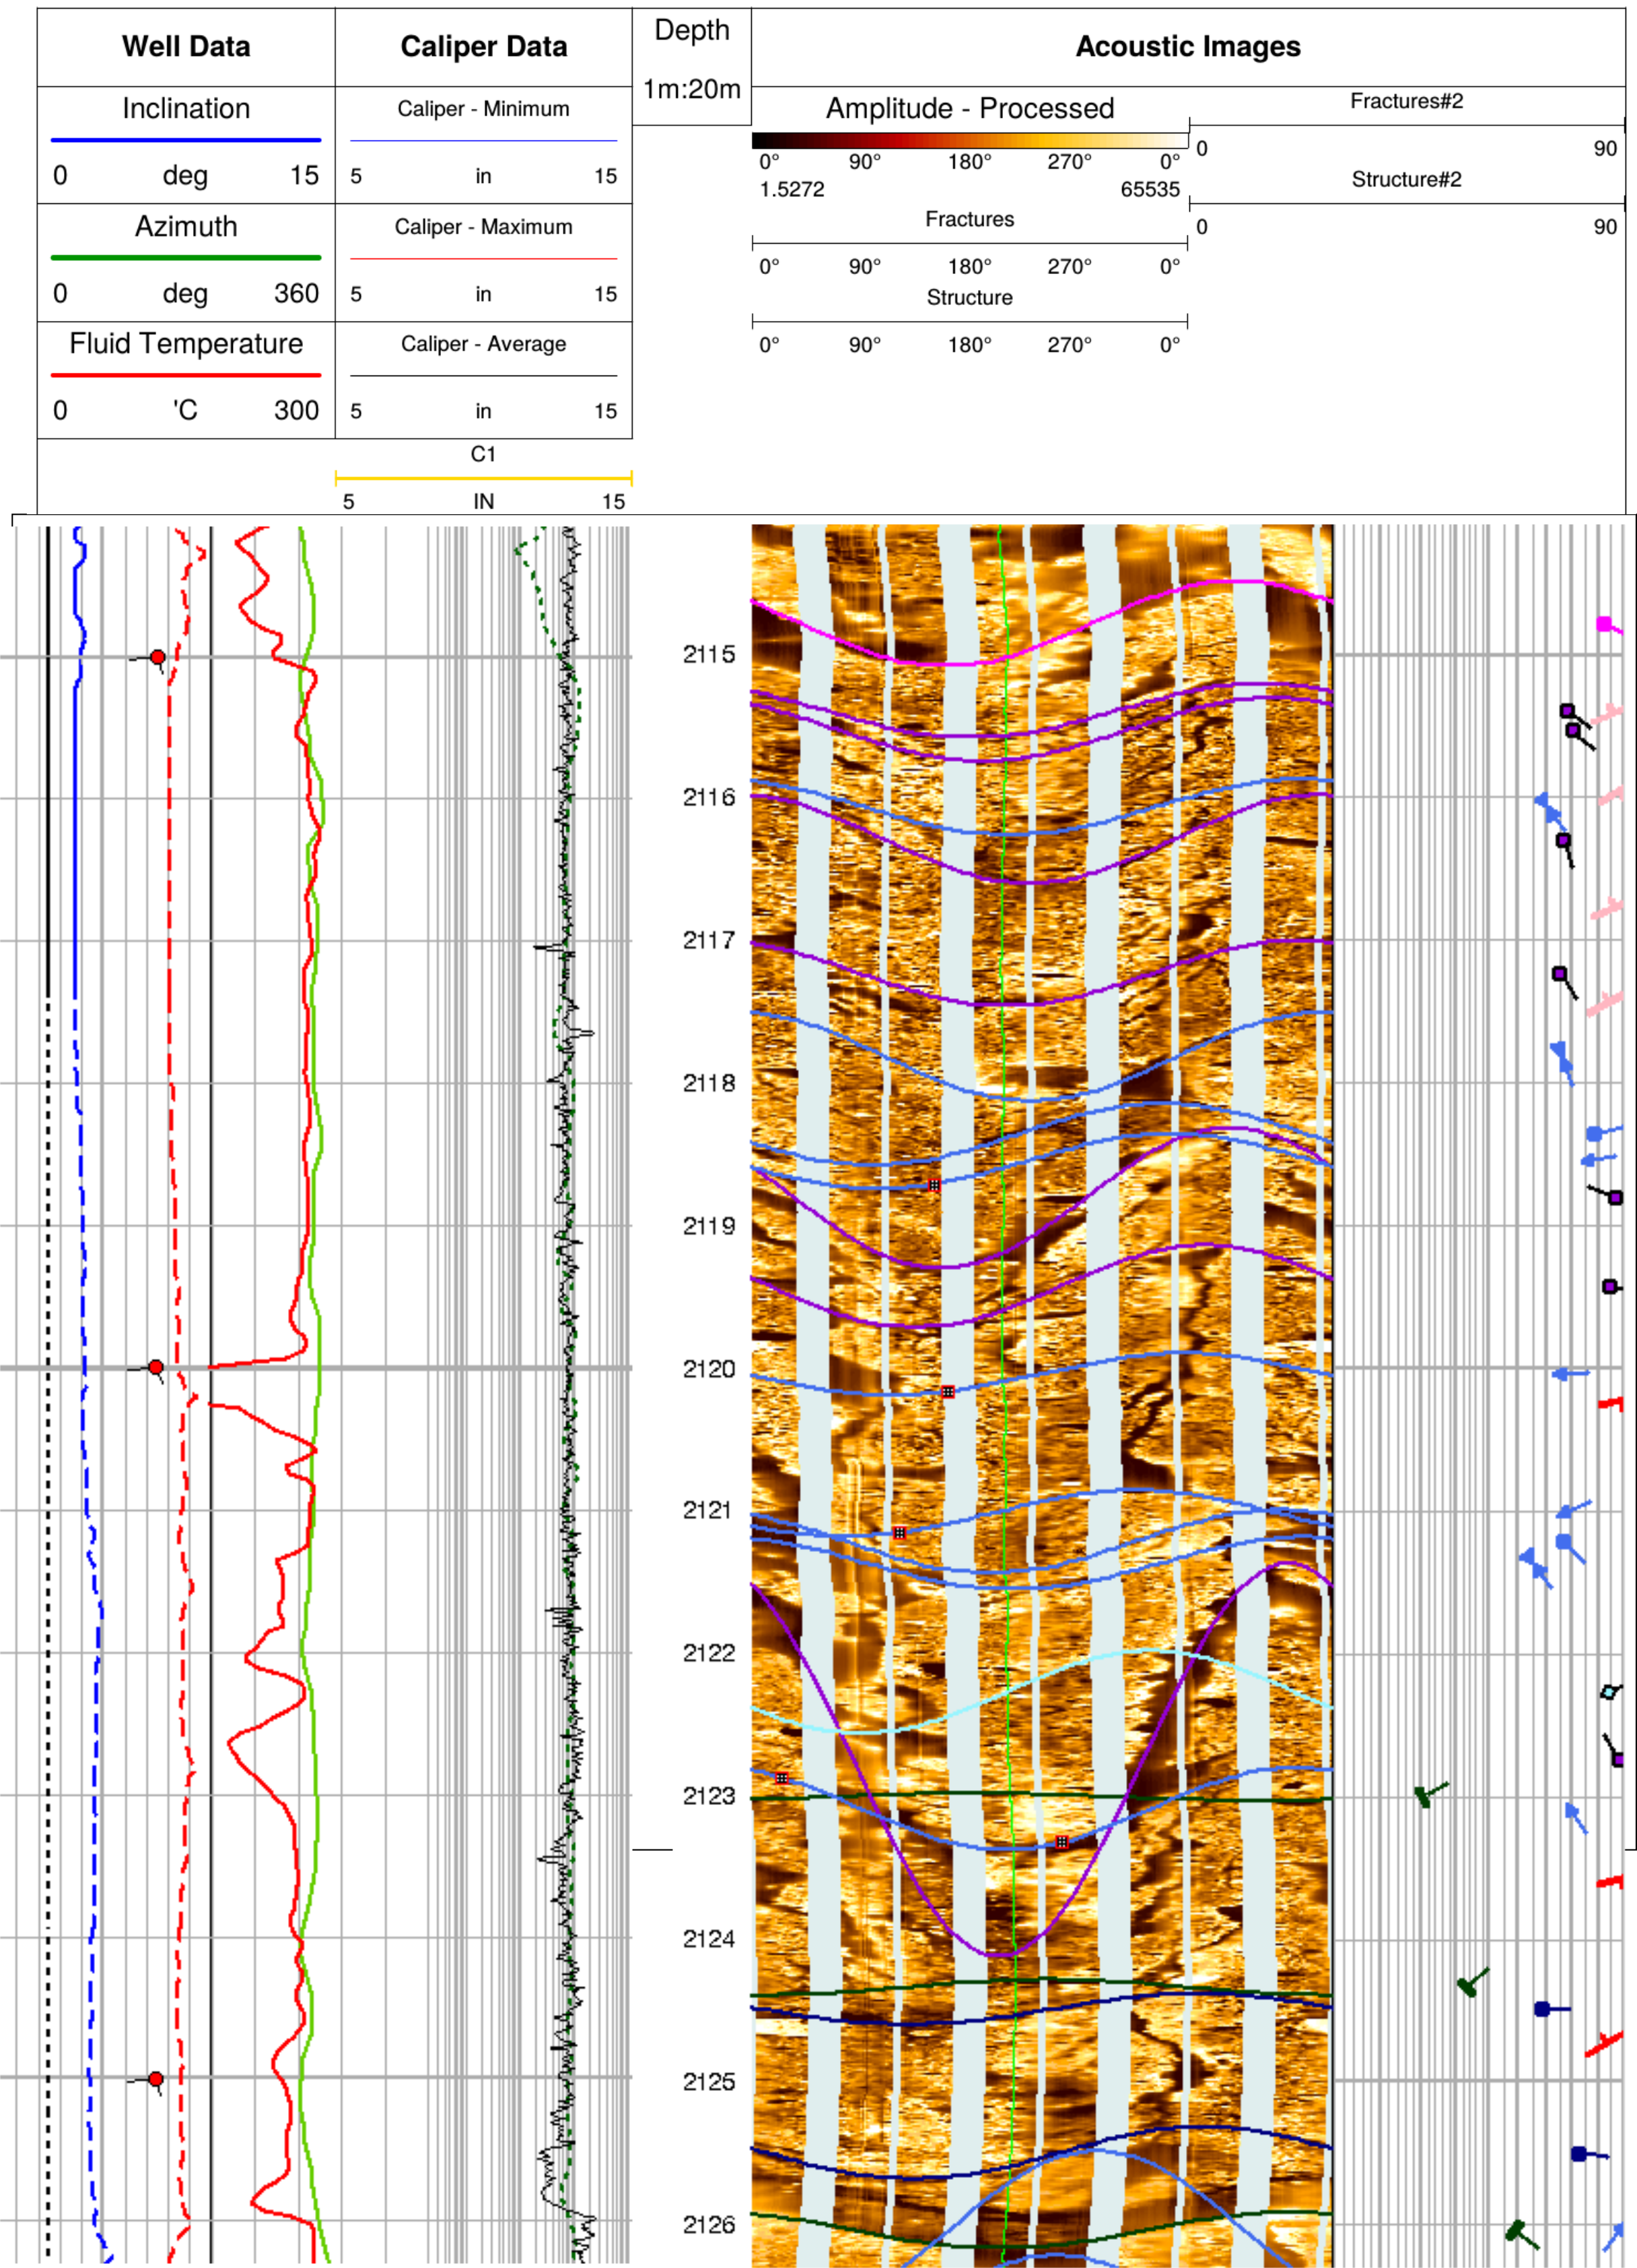
\includegraphics[width=0.70\columnwidth]{Chapter_2_Data/figures/FMI_example_mod/FMI_example_mod_original}
\caption{{Example interval from the FMI image of Ngatamariki well NM10, showing
interpreted fractures as well as other borehole data collected during
the survey.
{\label{746257}}%
}}
\end{center}
\end{figure}

\section{Methods}
\subsection{Earthquake Detection}
In order to construct a catalog of induced seismicity, earthquakes must first be detected in a noisy stream of data that contains few signals of interest. Detection is perhaps the most important task in the seismological workflow, yet the variety of methods employed to this end are imperfect and constantly being revised. In this thesis, we make use of two methods of detection, energy-based and correlation-based, the second built upon the first.

\subsubsection{Energy-based}\label{STA/LTA}
The energy released in an earthquake is proportional to the amplitude of the signal recorded at a given seismograph station \citep{stein_2000}. It is therefore intuitive that earthquakes can be detected by looking for changes in the amplitude of a single stream of seismic data, with the important caveat that the earthquake must have released a sufficient amount of energy to produce a signal of larger amplitude than the noise in the recorded data. The most ubiquitous technique for detecting earthquakes based on amplitude change is known as the STA/LTA method, whereby amplitudes in two overlapping windows of different duration are compared \citep{withers1998comparison}. The ratio of the average amplitude of the short-term (STA) window to the long-term (LTA) window defines the detection statistic and a detection (sometimes referred to as a `trigger') is recorded when the statistic exceeds a user-defined value.

A subsequent step in earthquake detection is known as `association', which involves the grouping of triggers from multiple seismographs into distinct events. When only one or two triggers occur across a network, local noise sources may have triggered these stations, whereas the presence of many triggers across the network at a similar time likely signifies the occurrence of a larger phenomenon, perhaps an earthquake.

As mentioned above, the energy-based detection for this thesis was undertaken by GNS Science using the SeisComP3 software package. Triggering and station magnitude calculation was done using the module \textit{scautopick} and event association using the module \textit{scautoloc}, yielding the starting catalog for the correlation based detection undertaken next.

\subsubsection{Correlation-based (matched filter)}\label{MF}
Where a stream of seismic data contains high levels of noise (e.g. in areas of extensive industrial activity) or a large number of signals, such as within an aftershock sequence, energy-based detection cannot realistically detect many of the events present in the data. Waveform cross-correlation has been used to overcome these deficiencies in finding known signals is such settings, and has been applied widely to problems including radar, digital communications and astronomy \citep[e.g.][]{Turin_1960,Abbott_2016}.

In seismology, matched filters have been adopted for use in finding a wide range of repeating and near-repeating signals that had eluded standard energy-based techniques, so long as the signal of interest was known. These applications include detection of local-to-regional scale crustal seismicity \cite{Schaff_2011,Dodge_2015,Chamberlain_2017}, low-frequency and non-volcanic tremor at plate boundaries \citep{Shelly_2007,Chamberlain_2014}, volcanic and volcano-tectonic signals \citep{Shelly_2016,Hotovec_Ellis_2018}, aftershock sequences \citep{Warren_Smith_2017} and explosions \citep{Gibbons_2006,Gibbons_2012}. In all instances, the known signal, be it an earthquake, radar pulse or nuclear explosion is referred to as the `template' and the discovered, previously unknown signals are termed `detections'. Throughout this thesis, we will also use the term `family' to mean all detections generated by a single template. Detections in the same family are shown for template 2012sora451121 in Figures \ref{434259} and \ref{233225}.\selectlanguage{english}
\begin{figure}[h!]
\begin{center}
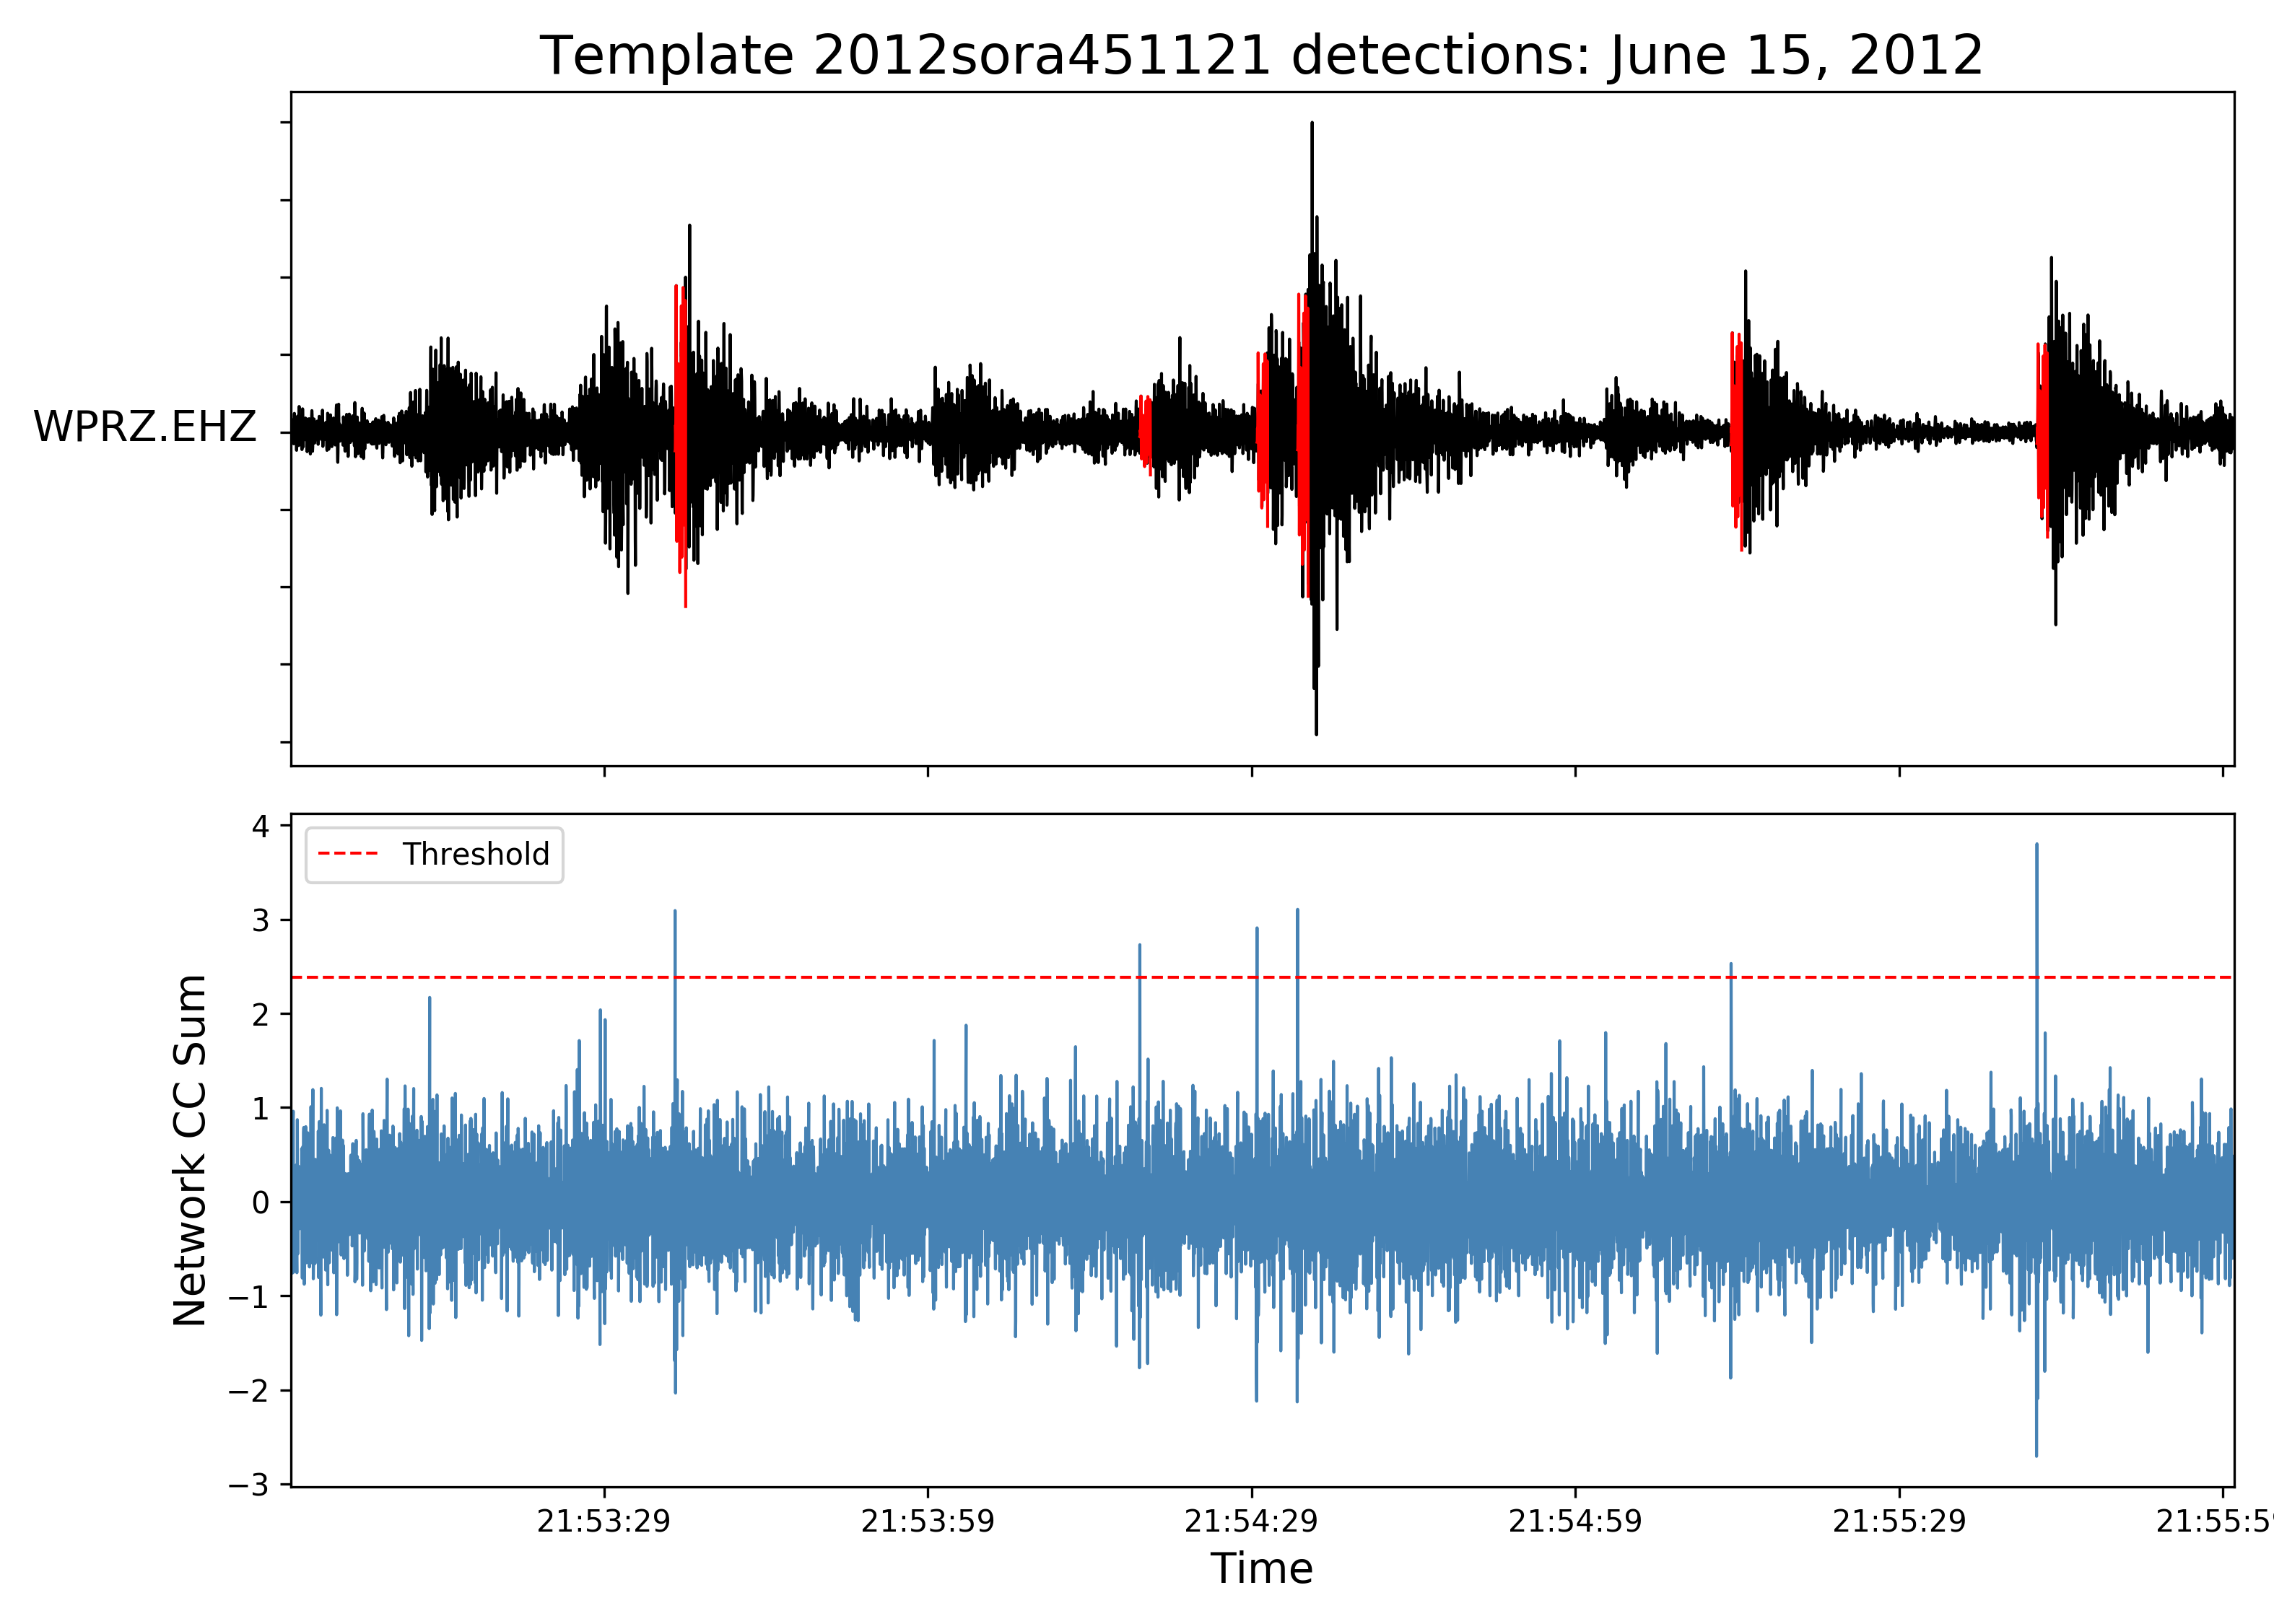
\includegraphics[width=0.70\columnwidth]{Chapter_2_Data/figures/2012sora451121_dets_cc_example/2012sora451121_dets_cc_example_original}
\caption{{Detections shown only at station WPRZ for template 2012sora451121 on 15
June 2012, during the stimluation of well NM08 (plot is three minutes
long). The top panel shows template waveforms (red) overlain on
continuous data (black). The bottom panel shows the cross-correlation
sum for the entire network in blue with the daily detection threshold
(MAD * 8) shown as a red dotted line.
{\label{434259}}%
}}
\end{center}
\end{figure}\selectlanguage{english}
\begin{figure}[h!]
\begin{center}
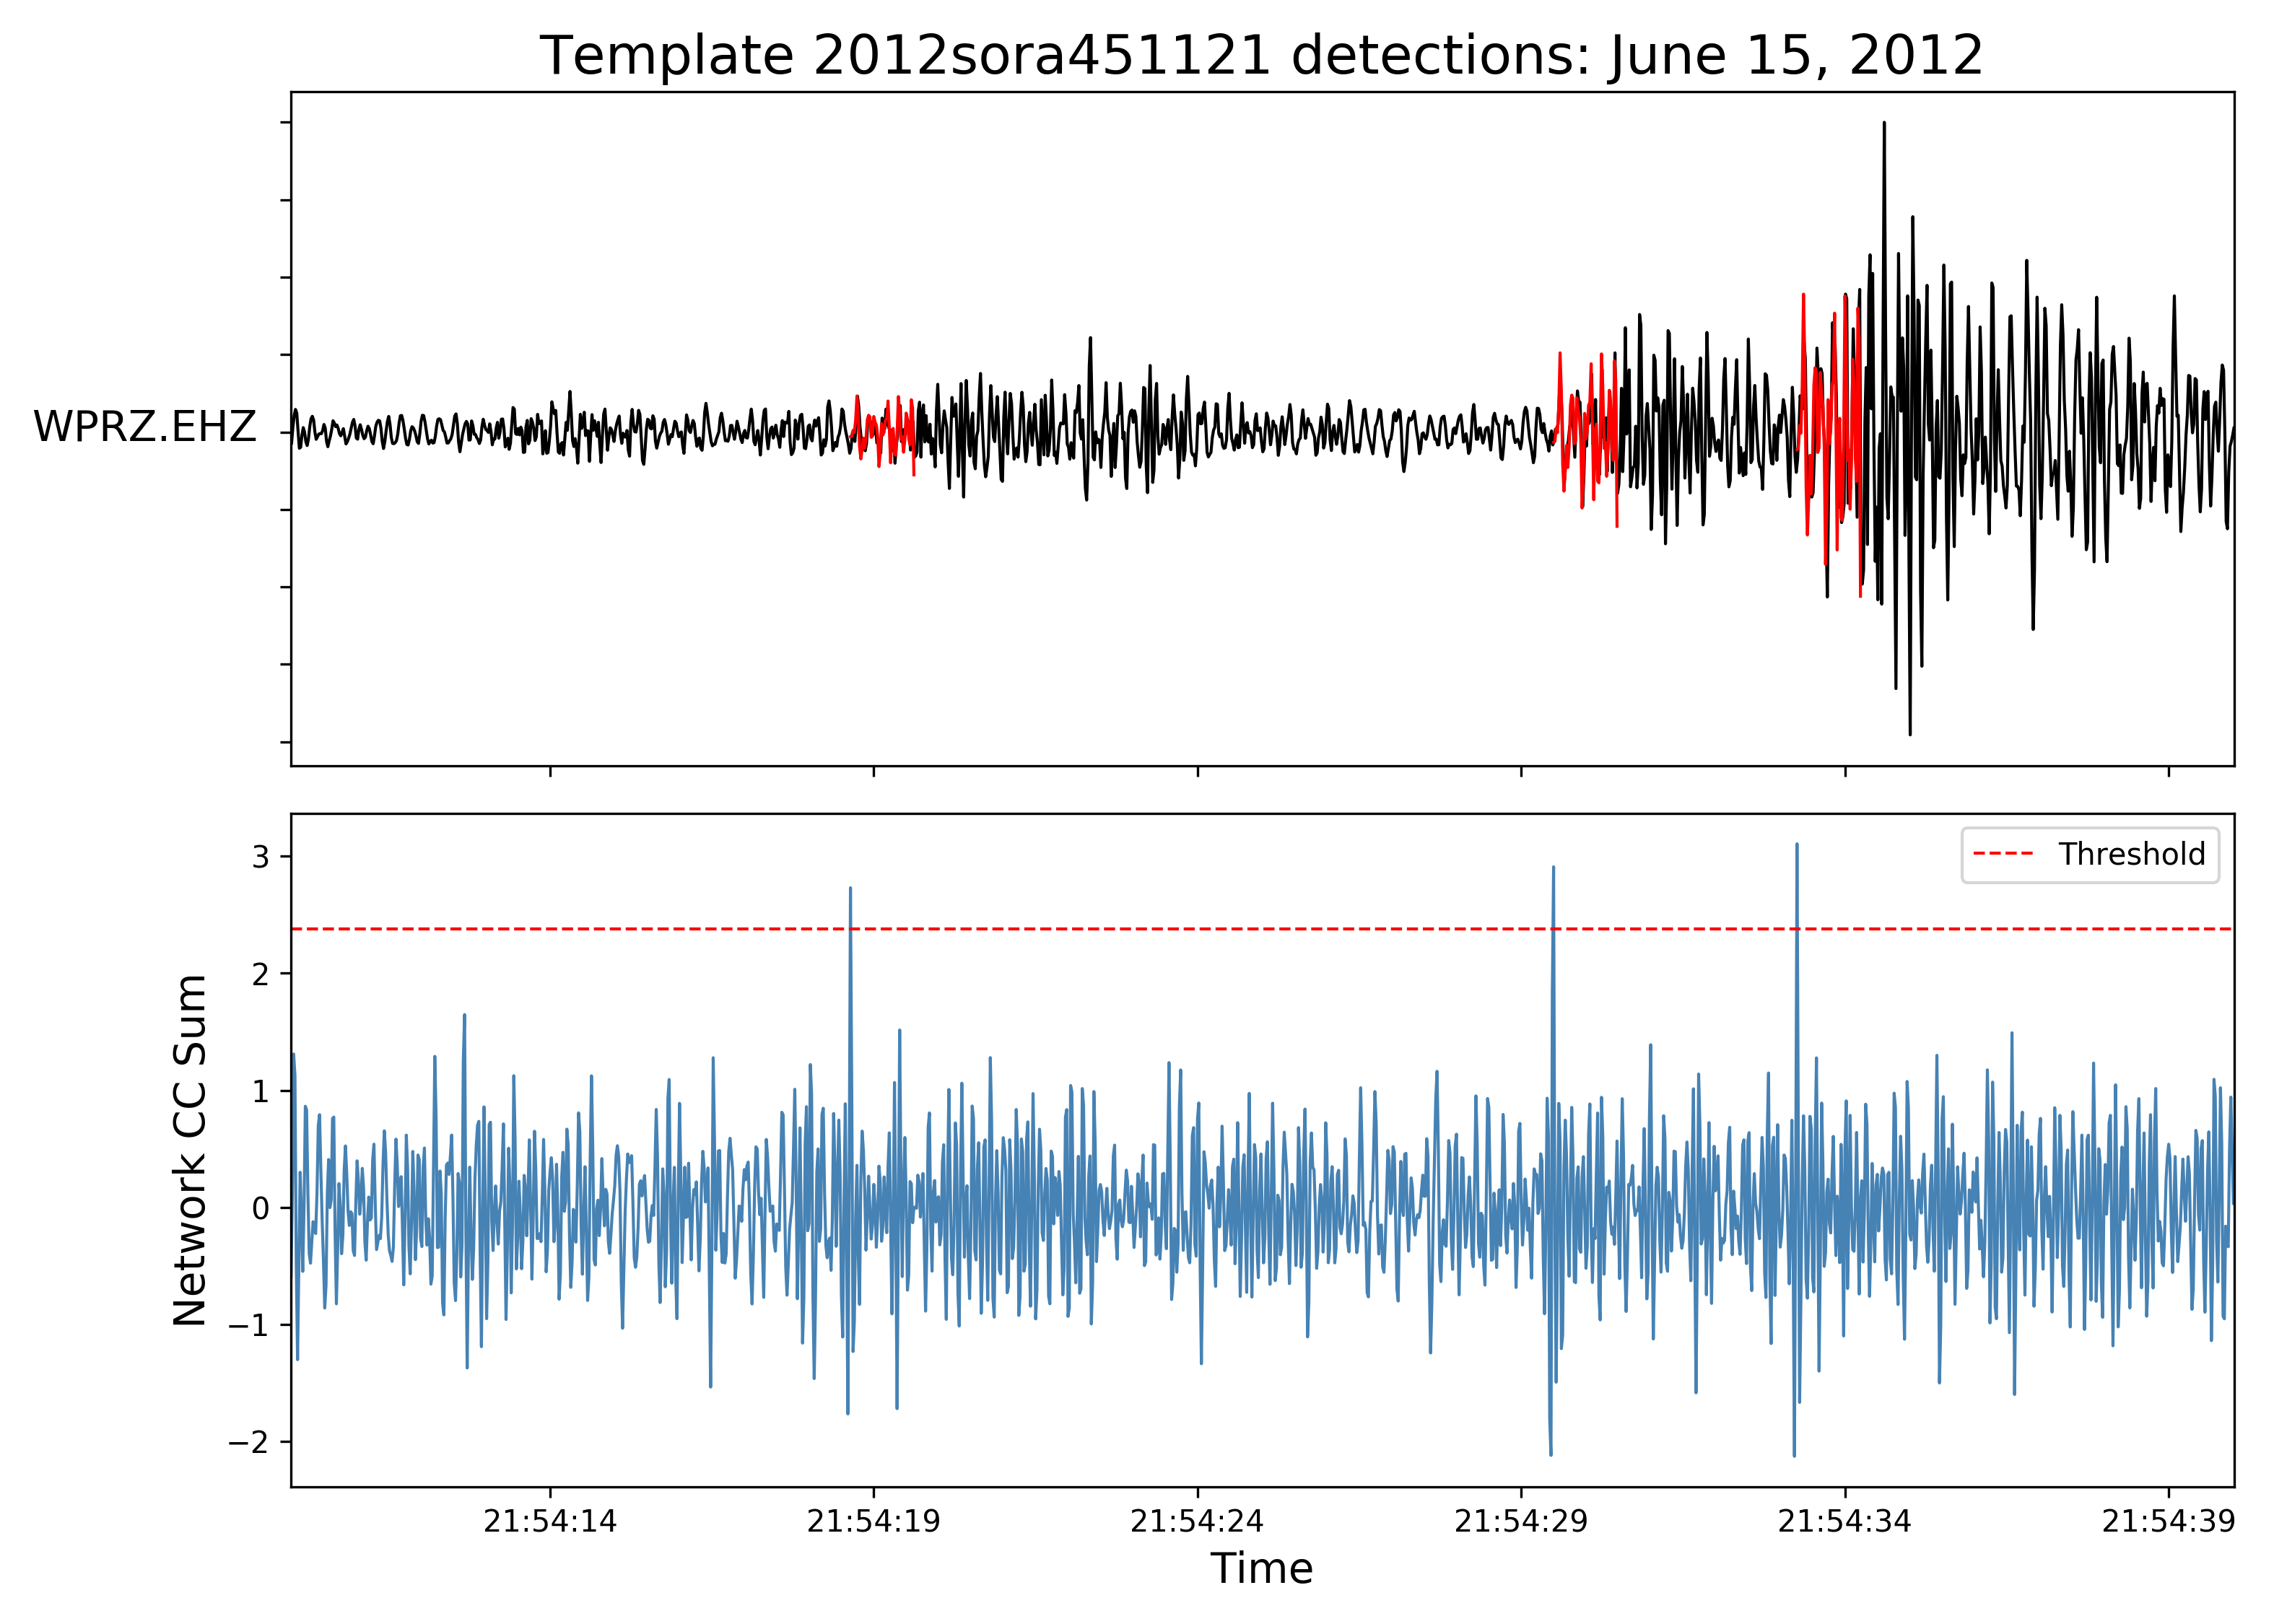
\includegraphics[width=0.70\columnwidth]{Chapter_2_Data/figures/2012sora451121_dets_cc_example_zoomed/2012sora451121_dets_cc_example_zoomed_original}
\caption{{The same plot as above, zoomed into only 30 seconds including three
detections in order to show the waveforms in more detail.
{\label{233225}}%
}}
\end{center}
\end{figure}


In this thesis, we use the matched-filter method to detect repeating and near-repeating, shallow (\textless10km depth) crustal seismicity at the Rotokawa and Ngatamariki geothermal fields using the GNS-detected catalog described above as template events. The cross correlation between a template event at a single station and the continuous seismic data being searched is described by the following equation \citep{Chamberlain_2017}:

\begin{equation}
R(x) = \frac{\sum_{x'=0}^{x+w_{x}}(T'(x') \cdot I'(x + x'))}{\sqrt[]{\sum_{x'=0}^{x+w_{x}}(T'(x')^2 \cdot \sum_{x'=0}^{x+w_{x}}I'(x+x')^2}}
\end{equation}

Here $I'$ represents the continuous seismic data of interest and $T'$ represents the template earthquake. $x$ represents the sample in the continuous data between sample $0$ and sample $(N_{x} - w_{x})$, where $N_{x}$ is the length of the continuous data being searched and $w_{x}$ is the length of the template. $x'$ is the position within the window over which the correlation is being calculated.

This cross-correlation coefficient at each seismograph station is then summed to yield the network detection statistic (blue curves, Figures \ref{434259} and \ref{233225}). The threshold for declaring a detection is calculated as the median absolute deviation (MAD) of the detection statistic for the entire period being searched (one day, for instance), multiplied by a user-defined value. In this thesis, we use a detection threshold of MAD $*$ 8, as suggested by \citep{Shelly_2007} (red dotted line, Figures \ref{434259} and \ref{233225}).

The template waveforms used in our matched-filter routine are one second long, starting 0.1 seconds before the P-pick, when present. During the energy-based detection, P-picks were only made on vertical channels. Therefore, templates consist of only vertical channel waveforms (e.g. red waveforms in Figure \ref{249518}, \ref{434259} and \ref{233225}). Horizontal channels are not used due to the large uncertainties for the automatic S-picks in the GNS Science catalog. However, a length of one second ensures that both the P- and S-arrival are included in the template for each event due to the short travel times between events and stations at the geothermal fields (Figure \ref{955268}). A length of one second also omits much of the coda, which is incoherent, even between highly-similar sources. This is especially apparent at Ngatamariki and Rotokawa, due to the highly-fractured reservoir, large variations in the volcanic geology (e.g.\ welded ignimbrites and ashfall deposits) and surface-deposit heterogeneity. After applying an anti-aliasing filter, waveforms were resampled at 50 Hz and filtered from 3.0 to 20.0 Hz to accommodate the high corner frequencies of events with event-station distances of \textless15 km. Continuous seismic data were processed in an identical manner to the templates.\selectlanguage{english}
\begin{figure}[h!]
\begin{center}
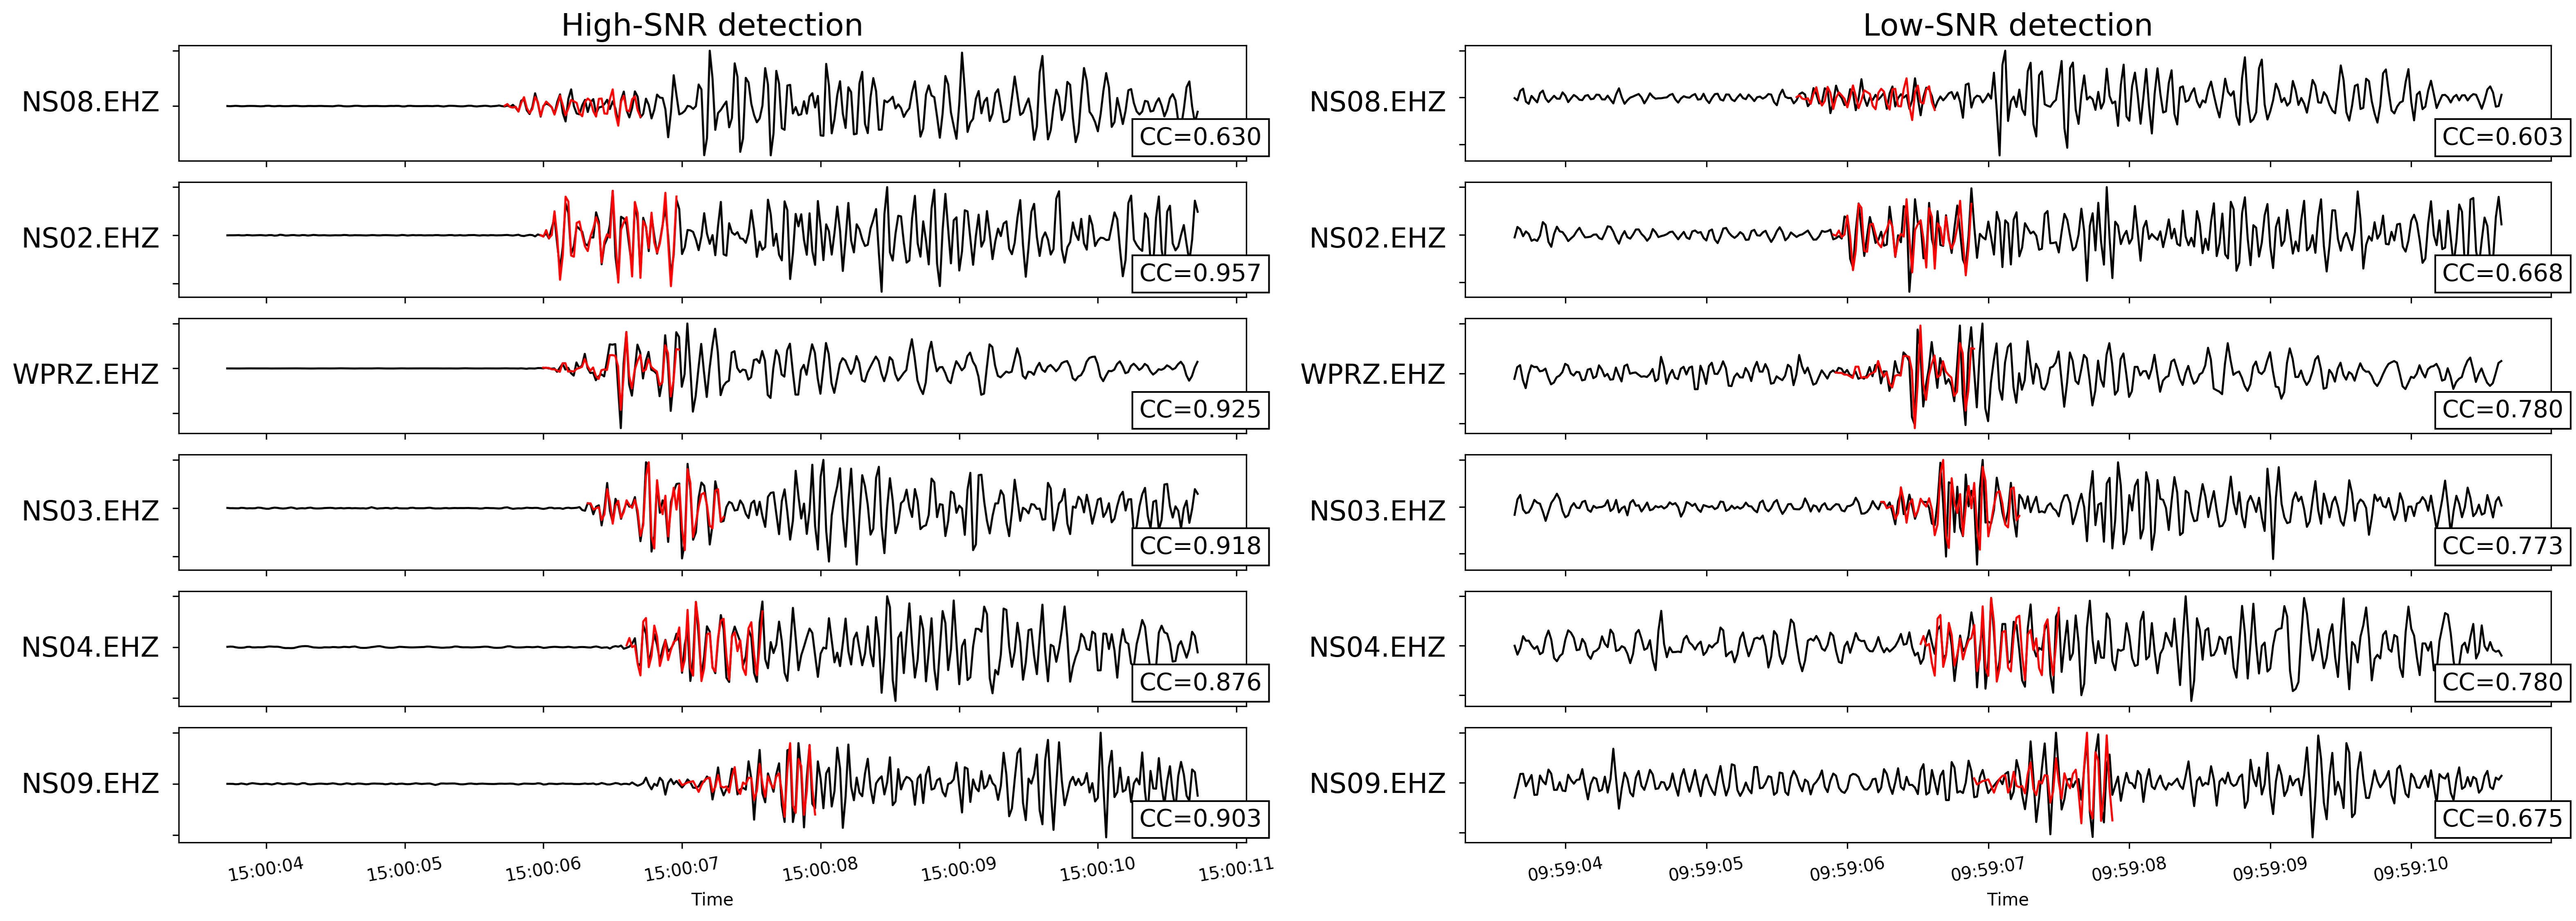
\includegraphics[width=0.98\columnwidth]{Chapter_2_Data/figures/det_example_publication/det_example_publication_original}
\caption{{Example detections of two events by template 2012sora469246
(signal-to-noise ratio of $\sim$50 and $\sim$3
respectively). The 1 s templates (in red) are overlain on 10 s of
continuous data around the time of detection (black). The ML 0.62
template event occurred on 22 June 2012 and detected mostly events that
occurred during the stimulation of well NM08 between 6 June and early
July. The detection on the left represents a detection of a separate,
yet highly-similar, template event (template 2012sora469256) which
occurred approximately ten minutes after the template event shown here.
The detection on the right is a newly-detected event.
{\label{249518}}%
}}
\end{center}
\end{figure}

\subsection{Earthquake Location}
Once a signal has been detected, the most critical piece of information regarding the event is its location (or hypocenter), meaning its three-dimensional point of occurrence in space. The locations contained in an earthquake catalog reveal subsurface features such as faults or the geometry of a subducting slab, and spatio-temporal variations can reveal characteristics of dynamic triggering or fluid migration. The problem of determining an earthquake's location, in conjunction with its time of occurrence, can be forward modeled from estimated source parameters or inverse modeled from signal arrival times at a series of seismographs. The algorithms used to determine spatial location and origin time, collectively referred to solely as `location' here, can be broken into three groups.

\subsubsection{Linear methods}\label{linloc}
The most computationally efficient, and widely-used method for solving the non-linear location problem is to iteratively solve the forward problem posed in the following equation:

\begin{equation}
t_i = T + \frac{1}{v}\sqrt[]{(X - x_i)^2 + (Y - y_i)^2 + (Z - z_i)^2}
\end{equation}

where $t_i$ is the arrival time of the ray traveling between the earthquake and recording station $i$, $T$ is the source time of the earthquake, $(X, Y, Z)$ are the longitude, latitude and elevation of the earthquake and $(x_i, y_i, z_i)$ are the longitude, latitude and elevation of station $i$.

Using the above equation, the arrival time at each station can be calculated by `guessing' a starting location, $(X, Y, Z)$, and origin time, $T$. The difference between the known arrival time at a given station, ${t_i}^obs$, and the calculated arrival time, ${t_i}^calc$, (often referred to as the `misfit' or `time residual', $r_i$) defines the quality of the chosen starting location:

\begin{equation}
r_i = {t_i}^{calc} - {t_i}^{obs}
\end{equation}

Minimizing these residuals across a seismic network is the goal of all earthquake location approaches. The classical method used to solve the problem is an inverse approach, originally used by Geiger \citep{l1910,geiger1912probability}, whereby a system of equations taking the form:

\begin{equation}
r_i = \frac{\partial{t_i}}{\partial{X}}\Delta{X} + \frac{\partial{t_i}}{\partial{Y}}\Delta{Y} + \frac{\partial{t_i}}{\partial{Z}}\Delta{Z} + \Delta{t_0}\label{eq:3}
\end{equation}

is solved iteratively until some condition, typically a threshold misfit value or location adjustment, is met. $(\Delta{X}, \Delta{Y}, \Delta{Z}, \Delta{t_0})$ are the adjustments in the starting location parameters between iterations and the partial derivatives are expressed as follows:

\begin{equation}
\frac{\partial{t_i}}{\partial{X}} = \frac{X - x_i}{vS}
\end{equation}
\begin{equation}
\frac{\partial{t_i}}{\partial{Y}} = \frac{Y - y_i}{vS}
\end{equation}
\begin{equation}
\frac{\partial{t_i}}{\partial{Z}} = \frac{Z - z_i}{vS}
\end{equation}

where $S$ represents the length of the source-receiver path.

Geiger's original method solved the problem via a least-squares approach, although many other methods have been proposed and used since, including adding damping parameters and solving via singular-value-decomposition \citep{thurber1985nonlinear}.

For real-world scenarios, the above equations oversimplify the problem of earthquake location because they assume the velocity of the subsurface is homogeneous. For most locations where earthquakes occur, the substrate is heterogeneous, consisting of horizontal layers (as the simplest case) and growing in complexity to include strong lateral heterogeneities as well (faults, for example). This velocity heterogeneity is approximated by a velocity model, which expresses velocity changes with depth (1-dimensional) and sometimes with geographic location as well (2- and 3-D cases).

For this thesis, the original linearized locations are calculated in SeisComP3 via the algorithm of \citet{Lee_1972}, which uses a step-wise regression approach, and a velocity model calculated for the entire Taupo Volcanic Zone \citep{Sherburn_2003}. For further relocations, we use a simple, 1-dimensional velocity model provided by \citet{sewell2017} specifically for our seismic network (Table \ref{vmod}).\selectlanguage{english}

\begin{table}
\centering
\begin{tabular}{cc}
    {Layer top (km)} & {$V_{P}$ (km/s)} \\ \midrule
    -0.6  & 1.9 \\
    0.2  & 2.6  \\
    1.0  & 3.5  \\
    1.5  & 3.6  \\
    2.0  & 3.9   \\
    3.0  & 4.9  \\
    5.0  & 5.4  \\
    10.0  & 5.81  \\
    20.0  & 6.9  \\
    50.0 & 7.43   \\
\end{tabular}
\caption{{Local 1-D velocity model for Ngatamariki and Rotokawa from VELEST inversions}}
\label{vmod}
\end{table}

\subsubsection{Non-linear methods}
In cases where the velocity model is poorly known, velocity structure is highly-variable, earthquake locations are shallow or are outside of the seismic network, the linearization approaches described above may be insufficient to address to location problem \citep{thurber1985nonlinear}. In this case, the second order terms corresponding to the first-order Taylor series expansion described in Equation \ref{eq:3} must be included. These terms are expressed as second-order partial differentials. For example:

\begin{equation}
\frac{\partial^{2}{t}}{\partial{Z}^{2}} = \frac{1}{vS}\left[1 - \frac{(Z - z_{i})^{2}}{S^2}\right]
\end{equation}

\begin{equation}
\frac{\partial^{2}t}{\partial{Y}\partial{Z}} = \frac{(Y - y_i)(Z - z_i)}{vS^3}
\end{equation}

\begin{equation}
\frac{\partial^{2}t}{\partial{X}\partial{Z}} = \frac{(X - x_i)(Z - z_i)}{vS^3}
\end{equation}

with the remaining latitude and longitude (x, y) terms taking similar forms to those above.

These second-order terms become especially important for shallow earthquakes located within a local seismic network and for short source-receiver paths, exactly the situation presented by the seismicity at Rotokawa and Ngatamariki. Given the high degree of nonlinearity for the seismic catalog at the geothermal fields, we have chosen to relocate both template and detected events with the program \textit{NonLinLoc} \citep{Lomax_2000}.

\textit{NonLinLoc} first computes the travel times to all stations for each node in a user-defined grid. As the user may then attempt to solve the location problem using a number of approaches, we selected the OctTree griding approach for all events at Rotokawa and Ngatamariki. The OctTree approach first calculates the probability that the source lies within any node in a coarse grid encompassing the entire, user-defined search area. This probability is proportional to the volume of the node and inversely proportional to the travel-time misfit calculated at its center \citep{Lomax_2000}. The highest-probability node is then divided into eight equal-volume sub-nodes and the process is repeated, dividing the most likely of the sub-nodes into eight and continuing this process until a threshold is reached and the maximum-likelihood hypocenter found. Typically, the threshold for halting the program is a minimum node volume. \textit{NonLinLoc} then samples the resulting OctTree structure of searched nodes in order to provide a representation of the location probability density function, which can then be used to characterize the uncertainty in the hypocenter solution \citep{Lomax_2000}.

\subsubsection{Relative location methods}
Perhaps the most significant uncertainty inherent in the location problem is that associated with the subsurface velocity structure. In an attempt to minimize the effect this uncertainty has on calculated locations, relative location methods have been developed, the most widely used of which is the double-difference method. Instead of minimizing the misfit between observed and calculated arrival times for a single event, double-difference techniques seek to minimize the misfit between the observed and calculated arrival time \textit{differences} between two paired events (hence, double-difference). The most popular of the double-difference location programs is \textit{HypoDD} \citep{Waldhauser_2000}, which attempts to solve the (oftentimes large) system of equations defining a web of interconnected pairs of events by minimizing the L2 norm of the double-differences.

A recent, alternative approach to the double-difference problem was developed by \citet{Trugman_2017}, which we use for the final relocations of the catalogs presented in this thesis. The \textit{GrowClust} algorithm makes use of the same data as \textit{HypoDD}, namely travel-time differences between pairs of events, as well as absolute travel time data and starting locations. However, instead of attempting to solve the entire system of equations defined by every event pair, \textit{GrowClust} creates a list of event pairs in order of descending similarity (defined as the sum of the cross-correlation coefficients between their common waveforms). It then relocates each event pair, or cluster pair where an event pair joins two preexisting clusters, relative to each other by minimizing the L1 norm (which is more robust to outliers than the L2 approach). Finally, \textit{GrowClust} also includes location error estimates via an iterative bootstrapping procedure that randomly resamples the input data and relocates the catalog. The location uncertainty is reported as the median absolute deviation of each event's location for each of the $n$ user-defined bootstrap iterations.

Application of these relative location techniques often proves imperative to obtaining precise locations, thus illuminating small-scale structures and migration of seismicity with time. Without these techniques, it can be difficult to interpret location results with any degree of confidence, especially at scales of \textless{10}km, as at Rotokawa and Ngatamariki.

\subsection{Magnitude calculation}
The calculation of earthquake magnitude is typically done in conjunction with its detection and location and is the final, key parameter required for analysis of any earthquake catalog. There are a number of ways in which earthquake magnitude is calculated, usually based on the measured maximum amplitude of a signal recorded at a number of seismograph stations, but can also be based on other measurements such as signal duration or full moment tensor inversion \citep{Kanamori_1983}. In this thesis, magnitudes for the GNS-located template events are reported at local magnitudes (M$_L$), and discussed in detail in Section \ref{GNS_cat}.

To compute the magnitude of the events detected by the matched filter,
we use the method described by \citet{Shelly_2016}, which uses pair-wise relative amplitudes between a template event and each of its detections to compute relative moments. This approach computes the relative amplitude, $\alpha$, as

\begin{equation}
\alpha = v[2] / v[1]
\end{equation}

where $v[2]$ and $v[1]$ are the second and first elements, respectively, of the first row of the 2$\times$2 matrix $V'$ in

\begin{equation}
M = U\Sigma V'
\end{equation}

where $M$ is the singular value decomposition of a data matrix containing both the template and the detected waveform on a single channel. The rows of $V'$ are the right singular vectors, which map the weight of the left singular vectors, $U$, to the original data vectors. Because the template and detected waveforms in the data matrix are inherently similar, the first left singular vector, $U_0$, should describe only a difference in amplitude between template and detection. The relative amplitude between the two events can therefore be estimated as the ratio of the second and first elements, $v[2]$ and $v[1]$, of the first row of $V'$.

We calculate relative amplitudes only when the cross-correlation coefficient between the template and detection exceeds 0.6 at any given station. Again, we note that template events only contain waveforms for the vertical channels. For those events recorded by a minimum of four stations exceeding the correlation threshold, we calculate the relative moment as the median of the relative amplitudes, following \citet{Shelly_2016}. We note that, because the relative amplitudes are calculated from two waveforms recorded at the same station, there is no need to remove the instrument response.

This approach has proven to be more robust in the presence of relatively dissimilar waveforms than the method of \citet{Rubinstein_2010}, which assumes high correlation coefficients between all events in a family (e.g.\ $\geq$0.85). At Rotokawa and Ngatamariki, scattering and attenuation effects produce waveforms exhibiting lower degrees of similarity than typical repeating or near-repeating seismicity (e.g.\ along the San Andreas \citep{Rubinstein_2010}).

We use the GNS Science $M_{L}$ (as described in Section \ref{GNS_cat}) to calibrate the relative moment calculations from the method above and produce $M_{L}$ estimates for the matched-filter detections. This is done by first converting the template $M_{L}$ to $M_{w}$ using the scaling relationship \citep{Ristau_2009}:

\begin{equation}
M_{L} = 0.88M_{w} + 0.73
\end{equation}

determined for locally detected, shallow New Zealand earthquakes and then converting to seismic moment using the equation \citep{Hanks_1979}:

\begin{equation}
M_w = \frac{2}{3}\log_{10}M_{0} - 9
\end{equation}

Knowing the relative moment of the template event from the procedure outlined above, we then determine the relationship between the relative moments and actual moment which allows us to convert relative moments to $M_w$ and then back to $M_L$ using the relationship of \citet{Ristau_2009}.

\subsection{Focal mechanisms}
The final step taken in developing the earthquake catalog presented here is the determination of earthquake focal mechanism solutions. The shear displacement on a fault is often represented as a point acted on by two perpendicular force couples (the so-called double-couple source), by ignoring any potential volumetric changes associated with the event \citep{stein_2000}. The energy radiated by such a double-couple source can be divided into four quadrants: two dilational and two compressional. At a given seismic station, the ground displacement from an arriving P-wave depends on which of the quadrants the path between the source and receiver emanated from. If that path emanated from a compressional quadrant the ground will move upwards, and if the path emanated from a dilational quadrant, the ground will move downwards. Therefore, by observing the pattern of first motion polarities (up or down) recorded across a seismic network, constraints can be placed on the orientation of the fault that slipped and the direction of slip associated with the corresponding earthquake \citep{stein_2000}.

A number of approaches have been developed to invert polarity recordings for the source properties of an earthquake, typically by forward modeling a large number of possible sources to find the mechanism which best fits the polarity observations \citep[e.g.][]{Reasenberg_1985,Hardebeck_2002}. The focal mechanism solutions presented in this thesis were calculated using the Bayesian approached developed by \citet{Walsh_2009}, which allows for the incorporation of known uncertainties in the input parameters (e.g. earthquake location and first arrival picks) and outputs a PDF of the focal mechanism solution.

\section{Appendices}
\subsection{Subspace Detection}
Although not incorporated into the results presented in the following chapters, we have undertaken work in developing and implementing functionality for additional detection techniques not detailed above. Specifically, we have developed functionality for the use of subspace detection of repeating and near-repeating seismicity, which we summarize below.

Matched-filter detection techniques are computationally expensive when applied
across large datasets. The expense is multiplied as more earthquakes are added
to the list of template events (referred to by \citet{Barrett_2014} as a `design set') and as larger seismograph networks with more channels of data are used. At the same time, it is important that a set of template events effectively represent the variety of sources present in a given study area or risk missing what might be important seismicity. Subspace detection has been used to address these considerations by expressing clusters of similar events as single matrices known as subspace detectors \citep[for example][]{Harris_2006a,Harris_2006, Barrett_2014,Chambers_2015}.

\subsubsection{Subspace detector design}
As outlined by \citet{Harris_2006a}, there are five main steps in constructing a series of subspace detectors from a catalog of earthquakes:
\begin{enumerate}
    \item Generate a distance matrix for all events by calculating, pairwise, the correlations between events in the catalog. Each element of the distance matrix, $D_{x, y}$ is equivalent to $1 - R(x, y)$ where $R(x, y)$ is the cross correlation value between events $x$ and $y$ (see Equation \ref{eq:3}).
    \item Cluster the events in the catalog based on this distance matrix. \citet{Harris_2006a} suggest a single-link agglomerative heirarchical clustering algorithm. Each cluster is then referred to as the design set for a single subspace detector.
    \item For each cluster, align the waveforms by cross correlation and trim the waveforms such that the first arrival occurs at the same point for each trace. Each waveform defines a column, $i$, of the data vector, $\underline{X}$.
    \item Calculate the orthonormal basis, $\underline{W}$, for the space defined by the design set, $\underline{X}$:

    \begin{equation}
    \underline{X} = \underline{W} \underline{\Sigma} \underline{V}^{T}
    \end{equation}
    
    \item Determine a satisfactory dimension $d$ such that the subspace defined by $\underline{W}_{d}$ approximates the waveforms in the design set:
    
    \begin{equation}
    \underline{X} \sim \underline{W}_{d} \underline{\Sigma}_{d} \underline{V}_{d}^{T}
    \end{equation}
    
    $W_{d}$ is our subspace detector and the matrix:
    
    \begin{equation}
    \underline{A}_{d} = \underline{\Sigma}_{d}\underline{V}_{d}^{T}
    \end{equation}
    
    gives the relative importance of each dimension, $d$, of $\underline{W}_{d}$ in describing the design set, $\underline{X}$.
\end{enumerate}

\subsubsection{Detection statistic}
Following the notation above, the detection statistic is defined as the following:

\begin{equation}
c[n] = \frac{\underline{x}_{p}^{T}[n]\underline{x}_{p}[n]}{\underline{x}^{T}[n]\underline{x}[n]}
\end{equation}

where $\underline{x}[n]$ is the data vector within the moving detection window and $\underline{x}_{p}[n]$ is the projection of $\underline{x}[n]$ onto the space defined by the subspace detector such that:

\begin{equation}
\underline{x}_{p}[n] = \underline{W}_{d}\underline{W}_{d}^{T}\underline{x}[n]
\end{equation}

This defines the ratio of the energy in the projected data $x_{p}[n]$ to the energy in the original data, $x[n]$ within the detection window $[n]$, which moves through the data period of interest one sample at a time.

\subsubsection{Determining a sufficient dimension}
Typically, the necessary number of dimensions in a subspace detector is determined empirically, using a plot such as Figure \ref{425783}, which shows the percentage of energy captured by the detector for all design set events with increasing dimensionality. For instance, \citet{Chambers_2015} stipulate that the desired dimension, $d$, is the smallest dimension for which the subspace detector, $\underline{W}_{d}$ captures an average of 90\% of the energy for all events in the design set, $\underline{X}$.\selectlanguage{english}
\begin{figure}[h!]
\begin{center}
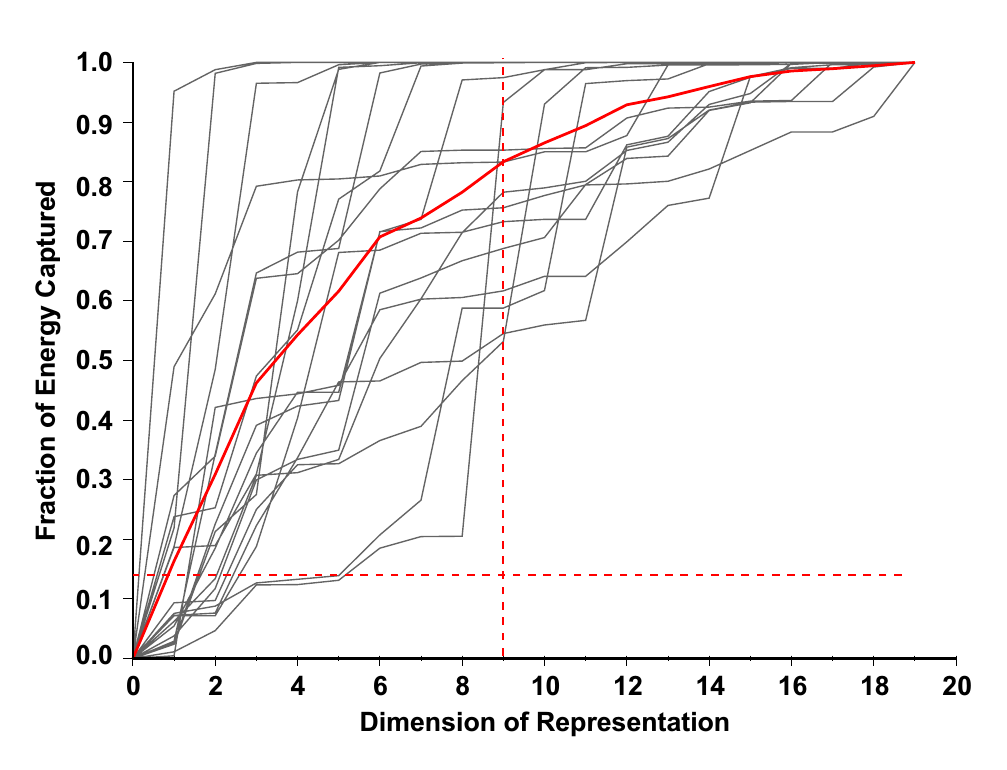
\includegraphics[width=0.70\columnwidth]{Chapter_2_Data/figures/Harris_2006_fig8/Harris_2006_fig8_original}
\caption{{Adapted from Harris et al. (2006), showing the percentage energy capture
by a subspace detector with increasing dimensionality. Gray lines show
energy capture for each event in the design set used to construct the
detector and the solid red line shows the average across all events. The
dotted red lines indicate the dimension (n=9) corresponding to an
average energy capture of 90\%.
{\label{425783}}%
}}
\end{center}
\end{figure}